\documentclass[11pt,draftcls,onecolumn,peerreview]{IEEEtran}
\bibliographystyle{plain}
\usepackage{graphicx}
\usepackage{amssymb}
\usepackage{amsmath}
\usepackage[bbgreekl]{mathbbol}
\DeclareMathOperator*{\argmax}{argmax}
\DeclareMathOperator*{\argmin}{argmin}
\usepackage[affil-it]{authblk}
\usepackage{paralist}
\usepackage{url}
\usepackage{tabularx}
\usepackage{color}
\usepackage{tikz}
\usepackage{tipa}\newcommand{\ipa}[1]{\textipa{#1}}
\usepackage{stackrel}
\usetikzlibrary{positioning,shadows,arrows,shapes,calc}
\setlength{\textwidth}{6.5in}
\setlength{\textheight}{9in}
\setlength{\oddsidemargin}{0in}
\setlength{\topmargin}{0in}

\title{ASR for Under-Resourced Languages from Probabilistic Transcription}

\author{Mark Hasegawa-Johnson$^1$,~\IEEEmembership{Senior~Member,~IEEE}
  Adrian KC Lee$^2$,~\IEEEmembership{Member,~IEEE}
  Ed Lalor$^3$,
  Preethi Jyothi$^1$,
  Daniel McCloy$^2$,
  Majid Mirbagheri$^2$,
  Giovanni di Liberto$^3$,
  Amit Das$^1$,
  Brad Ekin$^2$,
  Chunxi Liu$^4$,
  Vimal Manohar$^4$,
  Hao Tang$^5$,
  Nancy Chen$^6$,~\IEEEmembership{Senior~Member,~IEEE}
  Paul Hager$^7$,
  Tyler Kekona$^2$,
  and Rose Sloan$^8$}
\affil{1. University of Illinois, 2. University of Washington,
  3. Trinity College, Dublin, 4. Johns Hopkins University, 5. Toyota
  Technological Institute Chicago, 6. Institute for Infocomm Research,
  7. MIT, 8. Yale University}

\markboth{Draft, for review only}
{Hasegawa-Johnson \MakeLowercase{\textit{et al.}}: ASR for Under-Resourced Languages from Probabilistic Transcription}

\begin{document}
\maketitle

\begin{abstract}
In many under-resourced languages it is possible to find text, and it is possible to find speech, but transcribed speech suitable for training automatic speech recognition (ASR) is unavailable.  In the absence of native transcription, this paper proposes the use of a probabilistic transcription: a probability mass function over possible phonetic transcripts of the waveform.  Three sources of probabilistic transcription are demonstrated.  First, self-training is a well-established semi-supervised learning technique, in which a cross-lingual ASR first labels unlabeled speech, and is then adapted using the same labels.  Second, mismatched crowdsourcing is a recent technique in which non-speakers of the language are asked to write what they hear, and their nonsense transcriptions are decoded using noisy channel models of second-language speech perception.  Third, EEG distribution coding is a new technique in which non-speakers of the language listen to it, and their electrocortical response signals are interpreted to indicate probabilities.  ASR was trained in four languages with no transcribed training speech.  Adaptation using mismatched crowdsourcing significantly outperformed self-training, and both significantly outperformed a cross-lingual baseline.  EEG distribution coding and text-derived phone language models were both shown to improve the quality of probabilistic transcriptions derived from mismatched crowdsourcing.

\end{abstract}

\begin{IEEEkeywords}
Automatic speech recognition, Under-resourced languages, Crowdsourcing, EEG
\end{IEEEkeywords}

\ifCLASSOPTIONpeerreview
\begin{center} \bfseries EDICS Category: SPE-RECO \end{center}
\fi
% For peerreview papers, this IEEEtran command inserts a page break and
% creates the second title. It will be ignored for other modes.
\IEEEpeerreviewmaketitle

%%%%%%%%%%%%%%%%%%%%%%%%%%%%%%%%%%%%%%%%%%%
\section{Introduction}

\IEEEPARstart{A}{utomatic} speech recognition (ASR) has the potential to provide
database access, simultaneous translation, and text/voice messaging
services to anybody, in any language, dramatically reducing linguistic
barriers to economic success.  To date, ASR has failed to achieve its
potential, because successful ASR requires very large labeled
corpora. Current methods require about 1000 hours of transcribed
speech per language, transcribed at a cost of about 6000 hours of
human labor; the human transcribers must be computer-literate, and
they must be native speakers of the language being transcribed.  In
many languages, recruiting dozens of computer-literate
native speakers is impractical.

Instead of recruiting native transcribers in search of a perfect
reference transcript, this paper proposes the use of probabilistic
transcripts.  A probabilistic transcript is a probability mass
function, $\rho_\Phi(\phi)$, specifying, as a real number between $0$ and
$1$, the probability that any particular phonetic transcript $\phi$
is the correct transcript of the utterance.  Prior to this work,
machine learning has almost always assumed that the training dataset
contains either deterministic transcripts
($\rho_{DT}(\phi)\in\left\{0,1\right\}$, commonly called ``supervised
training'') or completely untranscribed utterances (commonly called
``unsupervised training,'' in which case we assume that $\rho_{LM}(\phi)$
is given by some {\em a priori} language model).  This article
proposes that, even in the absence of a deterministic transcript,
there may be auxiliary sources of information that can be compiled to
create a probabilistic transcript with entropy lower than that
of the language model, and that machine learning methods applied to
the probabilistic transcript are able to make use of its reduced
entropy in order to learn a better ASR.  In particular,
this paper considers three useful auxiliary sources of information:
\begin{enumerate}
\item SELF TRAINING: ASR pre-trained in other languages is used to
  transcribe unlabeled training data in the target language.
\item MISMATCHED CROWDSOURCING: Human crowd workers who don't speak
  the target language are asked to transcribe it as if it were a
  sequence of nonsense syllables.
\item EEG DISTRIBUTION CODING: Humans who do not speak the target
  language are asked to listen to its extracted syllables, and their
  EEG responses are interpreted as a probability mass function over
  possible phonetic transcripts.
\end{enumerate}



%%%%%%%%%%%%%%%%%%%%%%%%%%%%%%%%%%%%%%%%%%%%%%%%%%%%%%%%%%%%%%
\section{Background}

Consider the problem of developing speech technology in a language
with few internet-connected speakers.  Suppose we require that, in
order to develop speech technology, it is necessary first to have (1)
some amount of recorded speech audio, and (2) some amount of text
written in the target language.  These two requirements can be met by
at least several hundred languages: speech audio can be recorded
during weekly minority-language broadcasts on a local radio station,
and text can be acquired from printed pamphlets and literacy primers.
Recorded speech is, however, not usually transcribed; and the
requirement of native language transcription is beyond the economic
capabilities of many minority-language communities.

\subsection{Existing Approaches to ASR in Under-Resourced Languages}

Krauwer~\cite{Krauwer2003} defined an under-resourced language to be
one that lacks one or more of: stable orthography, significant
presence on the internet, linguistic expertise, monolingual tagged
corpora, bilingual electronic dictionaries, transcribed speech,
pronunciation dictionaries, or other similar electronic resources.
Berment~\cite{Berment2004} defined a rubric for tabulating the
resources available in any given language, and proposed that a
language should be called ``under-resourced'' if it scored lower than
10.0/20.0 on the proposed rubric.  By these standards, technology
methods for under-resourced languages are most often demonstrated on
languages that are not really under-resourced: for example, ASR may be
trained without transcribed speech, but the quality of the resulting
ASR can only be scientifically proven by measuring its phone error
rate (PER) or word error rate (WER) using transcribed speech.  The
intention, in most cases, is to create methods that can later be
ported to languages that truly lack resources.

The International Phonetic Alphabet (IPA~\cite{ipa1993}) is a set of
symbols representing speech sounds (phones) defined by the principle
that, if two phones are used in any language to make meaningful
linguistic contrasts (i.e., they represent distinct phonemes), then
those phones should have distinct symbolic representations in the IPA.
This makes the IPA a natural choice for transcriptions used to train
cross-language ASR systems, and indeed ASR in a new language can be 
rapidly deployed using acoustic models trained to represent every 
distinct symbol in the IPA~\cite{Schultz2001}.
However, because IPA symbols are defined phonemically, there is no
guarantee of cross-language equivalence in the acoustic properties of
the phones they represent. This problem arises even between dialects of
the same language: a monolingual Gaussian mixture model (GMM) trained on
five hours of Levantine Arabic can be improved by adding ten hours of
Standard Arabic data, but only if the log likelihood of cross-dialect
data is scaled by 0.02~\cite{Huang2012}.

Better cross-language transfer of acoustic models can be achieved, but only
by using structured transfer learning methods, including neural networks
(NN) and subspace Gaussian mixture models (SGMM).
NN transfer learning can be categorized as tandem, bottleneck,
pre-training, phone mapping, and multi-softmax methods.  In a tandem
system, outputs of the NN are Gaussianized, and used as features whose
likelihood is computed with a GMM~\cite{Hermansky2000}; in a
bottleneck system, features are extracted from a hidden layer rather
than the output layer. Both tandem~\cite{Stolcke2006} and
bottleneck~\cite{Vesely2012} features trained on other languages can
be combined with GMMs trained on the target language in order to
improve word error rate (WER).

A hybrid ASR is a system in which the NN terminates in a softmax
layer, whose outputs are interpreted as phone~\cite{Morgan95} or
senone~\cite{Dahl2012} probabilities.  Knowledge of the target
language phone inventory is necessary to train a hybrid ASR, but it is
possible to reduce WER by first pre-training the NN hidden layers with
multilingual data~\cite{Huang2013,Swietojanski2012}.  A hybrid ASR can be
constructed using very little in-language speech data by adding a
single phone-mapping layer to the output of the multilingual NN; the
phone mapping layer can be trained using a small amount of in-language
speech data~\cite{Sim2008}, even if context-dependent senones are
mapped instead of phones~\cite{Do2012}.  A multi-softmax system
integrates phone mapping into the original training procedure, by
training a network with several different language-dependent softmax
layers, each of which is the linear transform of a multilingual shared
hidden layer.  Multi-softmax systems have reduced WER in
tandem~\cite{Scanzio2008}, bottleneck~\cite{Vesely2012}, and
hybrid~\cite{Huang2013} ASR.

SGMM transfer learning uses language-dependent GMMs, each of which is
the linear interpolation of language-independent mean and variance
vectors.  SGMM can be combined with other methods for further
improvement, e.g., 16\% relative WER reduction was achieved in a Tamil
ASR by combining SGMM with an acoustic data normalization
technique~\cite{Mohan2014}, and further reductions were obtained in
Afrikaans by using bottleneck features in an SGMM~\cite{Imseng2014}.

%% Self-training is one of the three methods highlighted in the 
%% introduction. Doesn't it deserve its own sub-section?
Self-training is a class of semi-supervised learning techniques in
which ASR is first trained on labeled corpora in other languages, then
used to label data in the target language.  Self-labeled data in the
target language is then used to train or adapt the
ASR~\cite{Loof2009,Cetin2008}.  Self-training is most useful when the
in-language training data are first filtered, to exclude frames with
confidence below a threshold.  The posterior probability computed from
the ASR lattice is a useful confidence score~\cite{vesely2013-semi},
but it is also possible to learn an improved confidence score by
combining multiple sources of information~\cite{Vu2011b}.

Under-resourced languages often lack any pronunciation dictionary.  It
is possible to train a stable grapheme-to-phoneme transducer using a
dictionary with 15,000 entries, and in some languages a dictionary of
this size can be mined from sources such as
Wiktionary~\cite{Schlippe2014}.  In languages without any dictionary
of this size, it may be possible to approximate pronunciation by
treating each orthographic character as an acoustic 
model~\cite{Kanthak2002,Charoenpornsawat06,Gizaw2008,Le2009}.
Even an ambiguous G2P can often be disambiguated by the use of
context-dependent graphemic models~\cite{Kanthak2002}; if the number
of trigraphemes gets too large, acoustic models can be interpolated
within an eigentrigrapheme space~\cite{Ko2014}.  Optimal WER in
Standard Arabic was achieved by using phoneme-based pronunciations for
the most frequent 500 words, and grapheme-based pronunciations for all
less frequent words~\cite{Elmahdy2012}.  In Amharic, optimal WER was
achieved using a morpheme-based language model, combined with a hybrid
acoustic model space including both triphones and context-dependent
sylabic units~\cite{Tachbelie2014}.  In Hindi, optimal WER was
achieved using a one-to-one character-based grapheme-to-phoneme (G2P)
transducer (essentially a grapheme-based acoustic model), modified by
a very small set (3) of surface phonological
rules~\cite{Jyothi2015interspeech_hindi}.  The three rules were
proposed based on phonological descriptions of Hindi, then applied or
discarded in response to application probabilities learned using a
very small (200-word) pronunciation dictionary.


\subsection{Mismatched Crowdsourcing}
\label{sec:bgmc}

In~\cite{JHJ15a}, a methodology was proposed that bypasses the need
for native language transcription: mismatched crowdsourcing sends target
language speech to crowd-worker transcribers who have no
knowledge of the target language, then uses explicit mathematical
models of second language phonetic perception to recover an equivalent
phonetic transcription (Fig.~\ref{fig:h2e_eg2}).  Majority voting is
re-cast, in this paradigm, as a form of error-correcting code
(redundancy coding), which effectively increases the capacity of the
noisy channel; interpretation as a noisy channel permits us to explore
more effective and efficient forms of error-correcting codes.

\begin{figure}[b!]\setlength{\textfloatsep}{3mm}
\begin{center}
  \tikzstyle{pre2}=[<-,>=stealth',thick, draw=black]
  \tikzstyle{post2}=[->,>=stealth',thick, draw=black]
  \begin{tikzpicture}[
      scale=\mytikzscale,
      boxed/.style={rectangle,thick, draw=black, text=black, rounded corners=1mm, text centered, text width=2.5cm},
      open/.style={text=black, text centered, text width=2.75cm},
      every node/.style={transform shape}      
    ]
    \node[open] (n0) at (-4.5,1) {$w=$Utterance-language words\\\vspace*{0.1in}$<$$\vcenter{\hbox{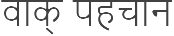
\includegraphics[width=1in]{../figs/vaakpahachaan.png}}}$$>$};
    \node[boxed] (n1) at (-0.75,1) {Pronunciation FST,\\$\rho(\phi|w)$} 
    edge[pre2](n0);
    \node[boxed] (n2) at (2.5,1) {Misperception FST,\\$\rho(\psi|\phi)$}
    edge[pre2] (n1);
    \node[boxed] (n3) at (5.75,1) {Phoneme-to-grapheme FST, $\rho(\lambda|\psi)$}
    edge[pre2] (n2);
    \node[open] (n4) at (9,1) {$\lambda$: Annotation-language orthography\\$<$vak paychan$>$} 
    edge[pre2](n3);
    \node[open] (n5) at (1,-1.5) {$\phi=$Utterance phones\\\ipa{[va:k p@H@tSa:n]}};
    \node[open] (n6) at (4,-1.5) {$\psi=$Perceived phones\\\ipa{[vAk p\textsuperscript{h}eItSAn]}}; 
  \end{tikzpicture}\\
\end{center}
\setlength{\abovecaptionskip}{0pt}
\caption{Mismatched Crowdsourcing: crowd workers on the web are asked
  to transcribe speech in a language they do not know.  Annotation
  mistakes are modeled by a finite state transducer (FST) model of
  utterance-language pronunciation variability (reduction and
  coarticulation), composed with an FST model of non-native speech
  misperception (mapping utterance-language phones to
  annotation-language phones), composed with an inverted
  grapheme-to-phoneme (G2P) transducer.}
\label{fig:h2e_eg2}
\end{figure}

Assume that cross-language phone misperception is a finite-memory
process, and can therefore be modeled by a finite state transducer
(FST).  The complete sequence of representations from utterance
language to annotation language can therefore be modeled as a noisy
channel represented by the composition of up to three consecutive FSTs
(Fig.~\ref{fig:h2e_eg2}): a pronunciation model, a misperception
model, and an inverted grapheme-to-phoneme (G2P) transducer.  The
pronunciation model is an FST representing processes that distort the
canonical phoneme string during speech production, including processes
of reduction and coarticulation.  The misperception model represents
the mapping of the uttered phone string (in symbols matching the
phone set of the spoken language) to the perceived phone string (in
symbols matching the phone set of the annotation language).  Finally,
the transcriber maps heard phones to nonsense words in the annotation
language; the mapping from phones to orthography is an inverted G2P.

%Preliminary experiments in mismatched crowdsourcing were carried
%out\cite{JHJ15a} using Hindi speech excerpts extracted from
%podcasts~\cite{SBS}.  Approximately one hour of speech was extracted
%from the podcasts (about 10000 word tokens in total) and phonetically
%transcribed by a Hindi speaker. The data were then segmented into very
%short speech clips (1 to 2 seconds long). The crowd workers were asked
%to listen to these short clips and provide English text, in the form
%of nonsense syllables, that most closely matched what they heard. The
%English text ($\lambda$) was aligned with the Hindi phone transcripts
%($\phi$) using a learned transducer, $\rho(\lambda|\phi)$, called a
%misperception G2P because it replaces both the misperception and G2P
%transducers from Fig.~\ref{fig:h2e_eg2}.  Fig.~\ref{fig:channelfst}
%shows a schematic diagram of the misperception G2P, with learned
%Levenshtein distances. This FST probabilistically maps each Hindi
%phone to either a single English letter or a pair of English
%letters. The FST substitution costs, deletion costs and insertion
%costs are learned to maximize $\rho(\lambda|\phi)$ using the
%expectation maximization algorithm (EM)~\cite{Dempster77}.
%\begin{figure}[b!]
%\centering
%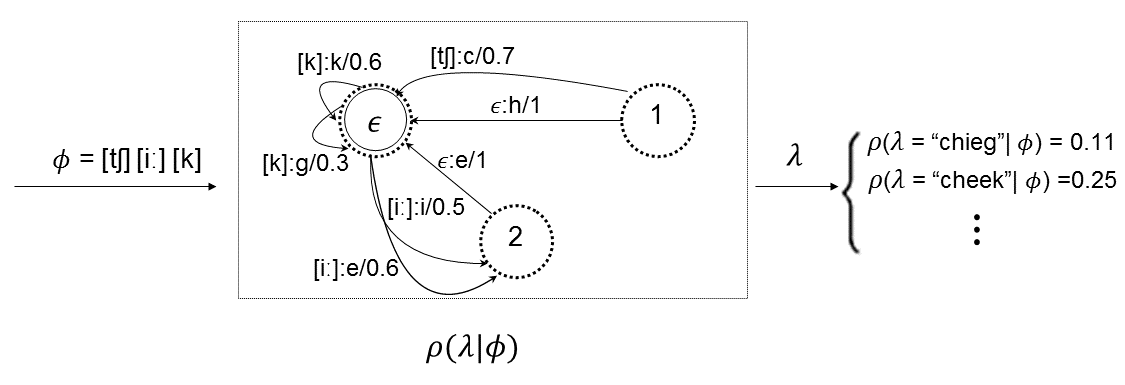
\includegraphics[width=\linewidth]{../figs/mismatchfst.png}
%\caption{Mismatch FST model of $\rho(\lambda|\phi)$, the probability
%  of English transcription $\lambda$ given Hindi phone sequence
%  $\phi$.  Figure modified slightly
%  from~\cite{JHJ15a}.\label{fig:channelfst}}
%\end{figure}


\subsection{Electrophysiology of Speech Perception}

The human auditory system is sensitive to within-category distinctions
in speech sounds, but such pre-categorical perceptual distinctions may
be lost in transcription tasks, where listeners must filter their
percepts through the limited number of categorical representations
available in their native language orthography.  EEG distribution
coding is a proposed new method that interprets the electrical evoked
potentials of untrained listeners (measured by
electroencephalography or EEG) as a probability distribution
over the phone set of the utterance language
(Fig.~\ref{fig:eeg_paradigm}).  Transcribers, in this scenario, listen
to speech in both their native language and an unfamiliar non-native
target language, while their EEG responses are recorded.  From their
responses to English speech, an English-language EEG phone recognizer
is trained~\cite{Liberto15}.  Misperception probabilities
$\rho(\psi|\phi)$ are then estimated: for each non-native phone
$\phi$, the classifier outputs are interpreted as an estimate of
$\rho(\psi|\phi)$.

\begin{figure}\setlength{\textfloatsep}{3mm}
\setlength{\fboxsep}{0pt}%
\setlength{\fboxrule}{0.5pt}%
\begin{center}
  \begin{tikzpicture}[
      scale=\mytikzscale,
      boxed/.style={rectangle,thick, draw=black, text=black, fill=white, 
      	rounded corners=1mm, text centered, text width=2.5cm},
      every node/.style={transform shape}      
    ]
    \node[text width=1.5in, text centered, anchor=north] (label0) at (-5,2.75) {EEG response to foreign phones (epoched \& averaged)};
    \node[text width=2.5in, text centered, anchor=north] (label1) at (0,2.75) {EEG feature classifiers trained on feature-labeled English phones};
    \node (raweeg) at (-5,0) {\fbox{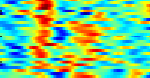
\includegraphics[width=1in]{../figs/avg-eeg.pdf}}};
    \node[boxed] (f0) at (-0.4,1.1) {\phantom{pd}};
    \node[boxed] (f1) at (-0.3,0.9) {\phantom{pd}};
    \node[boxed] (f2) at (-0.2,0.7) {\phantom{pd}};
    \node[boxed] (f3) at (-0.1,0.5) {\phantom{pd}};
    \node[boxed] (f4) at (0.0,0.3) {\phantom{pd}};
    \node[boxed] (f5) at (0.15,0.1) {\phantom{p}continuant\phantom{d}};
    \node[boxed] (f6) at (0.45,-0.4) {\phantom{p}sonorant\phantom{d}};
    \node[boxed] (f7) at (0.75,-0.9) {aspirated};
    \draw[->, thick] (-3.25,0) -- (-2,0);
    \draw[->, thick] (2,0) -- (3,0);
    \node[text width=1in, text centered] (label2) at (4.5,0) {\baselineskip=8pt Foreign phone misperception probabilities};
  \end{tikzpicture}\\
\end{center}
\setlength{\abovecaptionskip}{0pt}
  \caption{EEG responses are recorded while listeners hear speech in
    their native language.  For each listener, a bank of distinctive
    feature classifiers are trained.  Listeners then hear speech in an
    unfamiliar language, and their EEG responses are classified,
    estimating a listener-language probabilistic transcript of the
    non-native speech.}
  \label{fig:eeg_paradigm}
\end{figure}


%%%%%%%%%%%%%%%%%%%%%%%%%%%%%%%%%%%%%%%%%%%%%%%%
\section{Algorithms that Induce a Probabilistic Transcription}

Three different experimental sources were tested for the creation of a
PT.  Self-training is now well-established in the field of
under-resourced ASR; we adopted the algorithm of Vesely, Hannemann and
Burget~\cite{vesely2013-semi}.  Mismatched crowdsourcing used original
annotations collected using our own previously published
methods~\cite{JHJ15b}.  EEG was not used independently here, but
rather, was used to learn a misperception model applicable to the
interpretation of mismatched crowdsourcing.

\subsection{Self Training}
\label{sec:selftraining}

The method used for semi-supervised training is a modification of the
self-training approach described in \cite{vesely2013-semi}. In this
method, a multilingual DNN-HMM speech recognizer, trained languages
other than the target language, is used to decode unlabelled audio in
the target language.  As shown in Fig.~\ref{fig:fig_hager}, decoding
results in a posterior probability $\pi(\phi_m^\ell|x_t^\ell)$ for
each frame $x_t^\ell$ of audio in the target language.

\begin{figure}
  \centerline{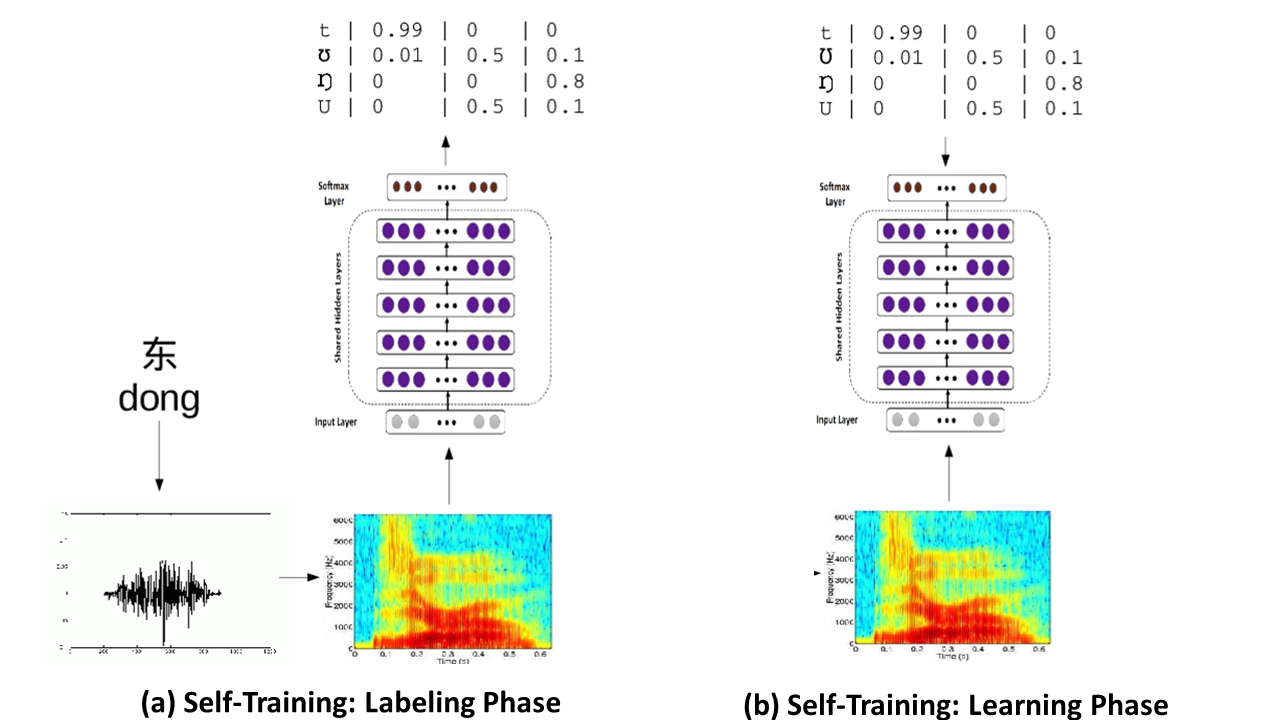
\includegraphics[width=5in]{../figs/fig_hager.png}}
  \caption{The self-training method of~\cite{vesely2013-semi} includes
    a labeling phase and a learning phase.  (a) Labeling phase: an ASR
    trained on other languages (here Cantonese) is used to compute
    posterior phone probabilities $\pi(\phi_t^\ell|x^\ell)$ in the
    test language (here Mandarin). (b) Learning phase: posterior phone
    probabilities are used as targets for DNN re-training.}
  \label{fig:fig_hager}
\end{figure}

We empirically found it better to use the posteriors as soft-targets
in frame cross-entropy training (Fig.~\ref{fig:fig_hager}). This is
different from the approach in \cite{vesely2013-semi}, which uses the
best path alignment as the target. Additionally, we scaled the amount
of transcribed data by 2 to create a good balance between transcribed
and untranscribed data as suggested in the original work.

The results on using this DNN are shown in Table \ref{tab:ptresult}. Although
semi-supervised training improves PER performance over multilingual DNN, it
still falls short of adaptation to probabilistic transcriptions (described in
Section \ref{sec:adaptation}). This is in spite of the untranscribed audio data
being several times larger than the probabilistic transcription data. Thus, we
show that mismatch transcripts can be more effective than ASR transcription for
training acoustic models.


\subsection{Mismatched Crowdsourcing}
\label{sec:MC}

%\begin{figure}
%  \centerline{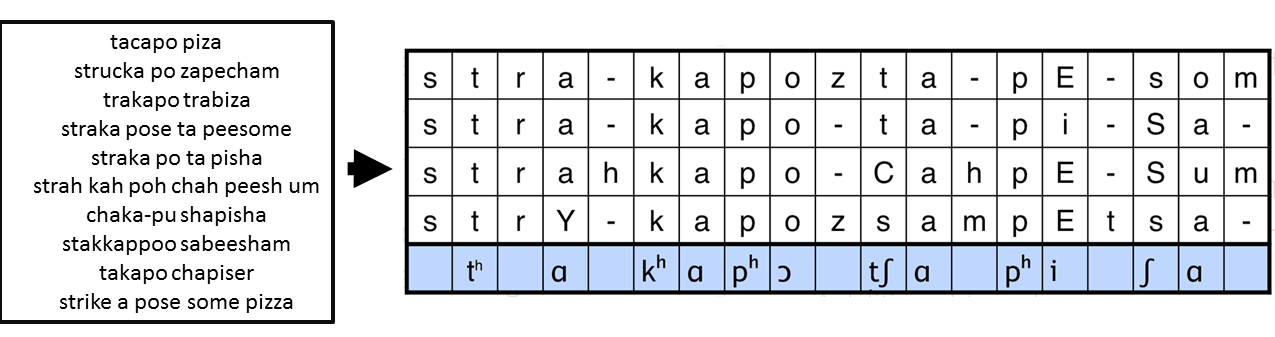
\includegraphics[width=5in]{../figs/fig_jyothi.png}}
%  \caption{In mismatched crowdsourcing, people who don't speak a
%    language (in this case Swahili) are asked to transcribe it using
%    nonsense syllables in the orthography of their own language (in
%    this case English).  There is a great deal of variability in their
%    responses (left), but information about the phonetic content of
%    the speech can be derived by merging the transcripts (top four
%    rows at right) and decoding using a model of non-native speech
%    perception (decoding result in the bottom row at right).}
%  \label{fig:mc}
%\end{figure}
%% comments: it's odd that all four of the illustrated transcripts begin
%% with the sequence [str], but the decoded result does not include the
%% [s] or the [r]. Perhaps it would be better to choose four transcripts
%% that vary more widely (and even indicate which orthographic strings
%% they correspond to) so that the derived result looks more plausible.
%% It is also odd that the formation of lambda involves choosing 5 best
%% MTs, but the figure shows 4 MTs.
%% Also, it is odd that pseudo-phonetic code is used in the transcripts
%% instead of IPA; IPA only occurs in the decoded result. Is there a
%% compelling reason for that?  Also, this figure is an excellent
%% candidate for vector graphic format rather than raster, since it's
%% all lines and text. I'm happy to help out with recreating figures in
%% vector format if that's desired.
%% Finally, I think this figure belongs after the following paragraph,
%% which could sensibly be merged into the opening paragraph of this
%% section. 

\begin{figure}[b!]\setlength{\textfloatsep}{3mm}
\begin{center}
  \tikzstyle{pre}=[<-,shorten <=3pt,>=stealth',thick, draw=black]
  \tikzstyle{post}=[->,shorten >=3pt,>=stealth',thick, draw=black]
  \begin{tikzpicture}[
      boxed/.style={rectangle,thick, draw=black, text=black, rounded corners=1mm, text centered, text width=5cm},
      state/.style={circle,thick, draw=black, text=black, text width=0.25cm},
      open/.style={text=black, text centered, text width=2.75cm},
    ]
    \node[boxed] (n0) at (0,0) {\begin{tiny}\begin{tabular}{c}$T$=Transcriptions\\\hline piza\\zapecham\\trabiza\\ta peesome\\ta pisha\\chah peesh um\\shapisha\\sabeesham\\chapiser\\some pizza\end{tabular}\end{tiny}};
    \node[boxed] (n1) at (6,0) {\begin{tiny}\begin{tabular}{c}$\rho(\lambda|T)=$Orthographic Confusion Network\\\hline\vspace{3cm}\end{tabular}\end{tiny}} edge[pre] (n0);
    \node[state] (g0) at (4,-0.25) {};
    \node[state] (g1) at (5.75,-0.25) {};
    \draw[post] (g0) -- (4.25,0.75) -- (5.25,0.75) -- (g1);
    \node at (4.75,1) {\tiny $<$t$>$$/0.4$};
    \draw[post] (g0) -- (4.25,-0.25) -- (5.25,-0.25) -- (g1);
    \node at (4.75,0) {\tiny $<$ch$>$$/0.4$};
    \draw[post] (g0) -- (4.25,-1.25) -- (5.25,-1.25) -- (g1);
    \node at (4.75,-1) {\tiny $<$s$>$$/0.2$};
    \node[state] (g2) at (7.5,-0.25) {};
    \draw[post] (g1) -- (g2);
    \node at (6.5,0) {\tiny $<$a$>$$/1.0$};
    \node[open] at (8.25,-0.25) {\ldots};
    \node[boxed] (n2) at (12,0) {\begin{tiny}\begin{tabular}{c}$\rho(\phi|T)=$Phone Confusion Network\\\hline\vspace*{3cm}\end{tabular}\end{tiny}} edge[pre] (n1);
    \node[state] (g10) at (10,-0.25) {};
    \node[state] (g11) at (11.75,-0.25) {};
    \draw[post] (g10) -- (10.25,0.75) -- (11.25,0.75) -- (g11);
    \node at (10.75,1) {\tiny \ipa{[t]}$/0.4$};
    \draw[post] (g10) -- (10.25,-0.25) -- (11.25,-0.25) -- (g11);
    \node at (10.75,0) {\tiny \ipa{[tS]}$/0.4$};
    \draw[post] (g10) -- (10.25,-1.25) -- (11.25,-1.25) -- (g11);
    \node at (10.75,-1) {\tiny \ipa{[s]}$/0.2$};
    \node[state] (g12) at (13.5,-0.25) {};
    \draw[post] (g11) -- (g12);
    \node at (12.5,0) {\tiny \ipa{[A]}$/1.0$};
    \node[open] at (14.25,-0.25) {\ldots};
  \end{tikzpicture}\\
\end{center}
\setlength{\abovecaptionskip}{0pt}
\caption{Probabilistic transcription from mismatched crowdsourcing:
  Transcripts $T$ are filtered to remove outliers, and merged to
  create a confusion network over orthographic symbols,
  $\rho(\lambda|T)$, from which the probabilistic transcription
  $\rho(\phi|T)$ is inferred. Example shown: Swahili speech,
  English-speaking transcribers.  Symbols in $<$$>$ are graphemes,
  symbols in $[]$ are phones, numbers are probabilities.}
\label{fig:mcmethods}
\end{figure}

The second set of PTs were computed by sending audio in the target
language to non-speakers of the target language (all transcribers were
speakers of American English, 30\% reported being monolingual), and
asking them to write what they hear.  Denote using $T$ the set of text
transcripts produced by these English-speaking crowd workers.
Mismatched transcripts must be converted into the form of a pmf over
target-language phone sequences, $\rho(\phi|T)$.  As an intermediate
step towards this goal, prior work~\cite{JHJ15b} developed techniques
to merge the transcripts in $T$ into a confusion network
$\rho(\lambda|T)$ over representative crowd-worker transcripts,
denoted $\lambda$ (Fig.~\ref{fig:mcmethods}).  Formation of
$\rho(\lambda|T)$ involves data filtering to remove outliers (based on
pair-wise string edit distance among transcripts), expansion of the
orthography to an alphabet that includes common digraphs (such as
$\lambda_m^\ell=<$ch$>$ in Fig.~\ref{fig:mcmethods}), and a weighted
voting scheme in which the weight of each transcript is proportional
to the frequency with which it matches the other transcripts.

Once transcripts have
been aligned and filtered to create the orthographic confusion network
$\rho(\lambda|T)$, they are then translated into a distribution over
phonemic transcriptions according to:
\begin{align}
  \rho(\phi|T) &=
  \sum_{\lambda} \rho(\phi|\lambda,T) \rho(\lambda|T) \notag \\
  &\approx \max_{\lambda}  \rho(\phi|\lambda) \rho(\lambda|T) \notag \\
  &= \max_{\lambda}  \left(\frac{\rho(\lambda|\phi)}{\rho(\lambda)}
  \rho(\phi)\right) \rho(\lambda|T) 
\label{eq:PT}
\end{align}
The terms other than $\rho(\lambda|T)$ in Equation~(\ref{eq:PT}) are
estimated as follows.  $\rho(\lambda)$ is modeled using a simple
context-free prior over the letter sequences in $\lambda$.
$\rho(\phi)$ is modeled using a bigram phone language model
%, trained
%on a corpus of Wikipedia text in the target language, converted into
%phone sequences as described in Section~\ref{sec:trainwithlm}.
$\rho(\lambda|\phi)$ is called the misperception G2P, as it maps to
graphemes in the annotation language, $\lambda$, from phones in the
utterance language, $\phi$.  Section~\ref{sec:eegchanmod} describes
methods that decompose $\rho(\lambda|\phi)$ into separate
misperception and G2P transducers, but it can also be trained directly
using
%the Carmel toolkit \cite{Knight99} as an FST mapping phones to letters
%based on
representative transcripts $\lambda$ (and their
corresponding native transcripts) for speech {\em in languages other
than the target language}. We assume that misperceptions depend more
heavily on the annotation language than on the utterance language, and
that therefore a model $\rho(\lambda|\phi)$ trained using a universal
phone set for $\phi$ is also a good model of $\rho(\lambda|\phi)$ for
the target language. Note that, while this assumption is not entirely
accurate, it is necessitated by the requirement that no native
transcriptions in the target language can be used in building any part
of our system.
%We also allow this FST to delete phones and insert letters.


\subsection{Estimating Misperceptions from Electrocortical Responses}
\label{sec:eegchanmod}

The misperception G2P described in Section~\ref{sec:MC} was estimated
using a combination of mismatched and deterministic transcripts of
non-target languages. However, With a small amount
of transcribed data in the utterance language, it is possible
to estimate the misperception G2P using electrocortical measurements
of non-native speech perception. In this approach, the misperception G2P
is decomposed into two separate transducers,
a misperception transducer $\rho(\psi|\phi)$, and an
annotation-language G2P $\rho(\lambda|\psi)$:
\begin{equation}
  \Pr(\lambda|\psi)=\sum_{\psi}\Pr(\lambda|\psi)\Pr(\psi|\phi)
\end{equation}
where $\phi$ is a phone string in the utterance language, $\psi$ is a
phone string in the annotation language, and $\lambda$ is an
orthographic string in the annotation language.  $\rho(\lambda|\psi)$
is an inverted G2P in the annotation language, e.g., trained on the
CMU dictionary of American English pronunciations~\cite{Lenzo1995}.
$\rho(\psi|\phi)$ is the mismatch transducer, specifying the
probability that a phone string $\phi$ in the utterance language will
be mis-heard as the annotation-language phone string $\psi$. 

In principle, the mismatch transducer could be computed empirically from
a phoneme confusion matrix, if experimental data on phoneme confusions
were available for all phones in the target language, and those data
were based on responses from listeners with the same language background
as the crowd worker transcribers. These goals are hard to meet. 
An alternative is to use distinctive feature representations
(originally proposed to characterize the perceptual and phonological
natural classes of phonemes~\cite{Jakobson52}) to predict misperceptions
based on differences between the distinctive feature values of 
transcription- and target-language phones. Given the assumption that 
every distinctive feature shared by phonemes $\phi$ and $\psi$ 
independently increases their confusion probability, their confusion 
probability can be expressed as
%\begin{equation}
%  \rho(\psi|\phi)\propto \exp\left(-\sum_{k=1}^K
%  w_k\delta\left(f_k(\psi)\ne f_k(\phi)\right)\right)
%  \label{eq:dfdist}
%\end{equation}
%where $f_k(\phi)$ is the $k^{\textrm{th}}$ feature of phoneme $\phi$,
%and $\delta(\cdot)\in\left\{0,1\right\}$ is the unit indicator
%function. 
\begin{equation}
  \rho(\psi|\phi)\propto \exp\left(-\sum_{k=1}^K
  w_k\right)
  \label{eq:dfdist}
\end{equation}
where $w_k(\phi)$ is the contribution of the $k^{\textrm{th}}$ feature in the 
misperception of the of phoneme $\phi$ as phoneme $\psi$. If a feature is 
perceived similarly across the two languages its contribution would be 
lower when when the two phonemes share the same value of that 
feature. The assumption of independence is a simplifying assumption,
given that many distinctive features have overlapping acoustic
correlates. For example, the frequencies of the {\em two} lowest
resonances of the vocal tract (the primary cues for vowel identity) are
determined by articulatory gestures of the lips, jaw and tongue that are
commonly represented by {\em three or more} distinctive features
(e.g., height, backness, rounding, and advanced tongue root). Moreover,
the weights $w_k$ will probably also depend on properties of the speaker
and listener (language, dialect, and idiolect), but data to train such a
rich model do not exist.

However, a reasonable approximate model can be learned by assuming that
$w_k$ depend only on information about the listener, which can be
incorporated via measurements of electrocortical activity. In particular,
the weights $w_k$ of the distinctive features can be set based on similarity
of electrocortical responses (measured using EEG) as determined by a
classifier trained on distinctive feature representations and
electrocortical responses to the listener's native language phones. Thus,
given a set of EEG response signals $y(\psi)$ recorded when a listener
hears audio corresponding to phoneme $\psi$ in the annotation
language, and supposing that $g_k(y(\psi))$ is the output of a binary
classifier trained on EEG responses to phones in his/her native language 
to detect the $k^{\textrm{th}}$ distinctive feature of phoneme $\psi$, 
as in~\cite{Liberto15}, then the contributions in Eq.~\ref{eq:dfdist} can be 
estimated as
\begin{equation}
  w_k = -\ln\Pr\left\{g_k(y(\psi))= f_k(\psi)\right\}
  \label{eq:eegdist}
\end{equation}


%%%%%%%%%%%%%%%%%%%%%%%%%%%%%%%%%%%%%%%%%%%%%%%%
\section{Algorithms for Training ASR Using Probabilistic Transcription}
%% from the point of view of the flow of data, it seems like section 
%% 4 (about generating PTs) should come before this section (which is
%% about adapting existing ASR system designs to use PTs)
% Good idea!  Done.

A deterministic transcription is a sequence of phone symbols,
$\phi^\ell =[\phi_1^\ell,\ldots,\phi_M^\ell]$ where $\phi_m^\ell$ is a
symbol drawn from the phone set of the utterance language.  We assume
that $\phi_m^\ell$ can be encoded using an IPA symbol~\cite{ipa1993}.
The superscript specifies that $\phi^\ell$ is the transcription of the
$\ell^{\textrm{th}}$ waveform in a database; the collection of all
transcriptions is $\phi=\left\{\phi^1,\ldots,\phi^L\right\}$.

%% the visible difference between regular and blackboard fonts is
%% barely noticeable in the typeset document. Is there an alternative
%% way of specifying sets, or a typeface that visually distinguishes
%% normal from blackboard variants more prominently?
% MH: mathbb seems to only distinguish roman letters, so let's try V_phi
A probabilistic transcription is a probability mass function (pmf)
over the set of deterministic transcriptions.  Capital letters
denote random variables, lowercase denote instances, and
blackboard font denote sets.  $\Phi^{\ell}_m$ is a random variable
whose instance is $\phi_m^\ell\in\mathbb{V}_\phi$, where $\mathbb{V}_\phi$
is the union of the set of IPA symbols with the null symbol
($\varnothing$), thus $\mathbb{V}_\phi =\left\{\right.\varnothing,$
\ipa{[a],[i],[2],[\ae],}$\left.\ldots\right\}$, with cardinality
$|\mathbb{V}_\phi|$ equal to one plus the number of distinct IPA
symbols.  Similarly, $\Phi^{\ell}$ is a random variable whose instance
is $\phi^{\ell}\in\mathbb{V}_\phi^*$, where $\mathbb{V}_\phi^*$ denotes
the set of all sequences composed of symbols in $\mathbb{V}_\phi$.  
Denote the probability of transcription $\phi^{\ell}$ as
$\rho_{\Phi^\ell}(\phi^{\ell})$, where the symbol ``$\rho$'' is
selected to emphasize that $\rho_{\Phi^\ell}(\phi^{\ell})$ is a
reference distribution---a distribution specified by the probabilistic
transcription process, and not dependent on ASR model
parameters.  The distribution label $\Phi^\ell$ is omitted when clear
from the instance label, e.g., $\rho_{\Phi^\ell}(\phi^\ell)$ may be
abbreviated as $\rho(\phi^\ell)$, but $\rho_{\Phi^\ell}(u)$ may not.
A deterministic transcription is a degenerate probabilistic
transcription, in which $\rho(\phi^\ell)\in\left\{0,1\right\}$.
%% comment: I'm guessing the choice of epsilon for the null phoneme is
%% related to its use representing the "empty string". Incidentally,
%% linguists use the mathematical "empty set" character (U+2205) to
%% represent a null phoneme (used in formulas for phonological rules
%% where sounds get deleted). It's not officially part of the IPA, but
%% might be a more natural choice (depending on the audience). See:  
%% https://en.wikipedia.org/wiki/Zero_%28linguistics%29 
%% also note that different variants of epsilon are being used in the 
%% main text (lunate variant) and in fig:liu1 (two-lobed variant).
%% If epsilon is retained, it should at least be the same epsilon
%% throughout.
% MH: OK, let's try empty set to see if it works...
A database consists of $L$ speech waveforms, each containing $T$
frames with $M$ associated phone labels, $M<T$.  Superscript denotes
waveform index, while subscript denotes frame or phone index.
Absence of either superscript or subscript denotes a collection, thus
$\Phi=\left\{\Phi^1,\ldots,\Phi^L\right\}$ (with instance value
$\phi=\left\{\phi^1,\ldots,\phi^L\right\}$) is the random variable
over all transcriptions of the database.  In all of the work described
in this paper, the probabilistic transcription is represented as a
confusion network~\cite{Mangu00}, meaning that it is the product of
independent symbol pmfs $\rho(\phi_m^\ell)$:
\begin{equation}
  \rho(\phi)=\prod_{\ell=1}^L\rho(\phi^\ell)=
  \prod_{\ell=1}^L \prod_{m=1}^M \rho(\phi_m^{\ell})
\end{equation}
The pmf $\rho(\phi^\ell)$ can be represented as a weighted
finite state transducer (wFST) in which edges connect states in a
strictly left-to-right fasion without skips, and in which the edges
connecting state $m$ to state $m+1$ are weighted according to the pmf
$\rho(\phi_m^\ell)$ (Fig.~\ref{fig:pt}).
\begin{figure}
\begin{center}
  \tikzstyle{pre}=[<-,shorten <=1pt,>=stealth',semithick,draw=black]
  \tikzstyle{post}=[->,shorten >=1pt,>=stealth',semithick,draw=black]
  \begin{tikzpicture}[
      state/.style={circle,thick, draw=black, text=black, text width=0.25cm},
    ]
    \node[state] (g0) at (0,0) {};
    \node[state] (g1) at (2,0) {};
    \draw[post] (g0) -- (0.5,1) -- (1.5,1) -- (g1);
    \node at (1,1.25) {\ipa{[a]}$/0.5$};
    \draw[post] (g0) -- (0.5,0) -- (1.5,0) -- (g1);
    \node at (1,0.25) {\ipa{[\ae]}$/0.4$};
    \draw[post] (g0) -- (0.5,-1) -- (1.5,-1) -- (g1);
    \node at (1,-0.75) {$\emptyset/0.1$};
    \node[state] (g2) at (4,0) {};
    \draw[post] (g1) -- (2.5,1.5) -- (3.5,1.5) -- (g2);
    \node at (3,1.75) {\ipa{[\"*b]}$/0.45$};
    \draw[post] (g1) -- (2.5,0.5) -- (3.5,0.5) -- (g2);
    \node at (3,0.75) {\ipa{[V]}$/0.35$};
    \draw[post] (g1) -- (2.5,-0.5) -- (3.5,-0.5) -- (g2);
    \node at (3,-0.25) {\ipa{[b]}$/0.10$};
    \draw[post] (g1) -- (2.5,-1.5) -- (3.5,-1.5) -- (g2);
    \node at (3,-1.25) {\ipa{[p]}$/0.10$};
    \node[state] (g3) at (6,0) {};
    \draw[post] (g2) -- (4.5,1) -- (5.5,1) -- (g3);
    \node at (5,1.25) {\ipa{[i]}$/0.7$};
    \draw[post] (g2) -- (4.5,0) -- (5.5,0) -- (g3);
    \node at (5,0.25) {\ipa{[e]}$/0.2$};
    \draw[post] (g2) -- (4.5,-1) -- (5.5,-1) -- (g3);
    \node at (5,-0.75) {$\emptyset/0.1$};
    \node[state] (g4) at (8,0) {};
    \draw[post] (g3) -- (6.5,1.5) -- (7.5,1.5) -- (g4);
    \node at (7,1.75) {\ipa{[a]}$/0.3$};
    \draw[post] (g3) -- (6.5,0.5) -- (7.5,0.5) -- (g4);
    \node at (7,0.75) {\ipa{[\ae]}$/0.3$};
    \draw[post] (g3) -- (6.5,-0.5) -- (7.5,-0.5) -- (g4);
    \node at (7,-0.25) {\ipa{[i]}$/0.2$};
    \draw[post] (g3) -- (6.5,-1.5) -- (7.5,-1.5) -- (g4);
    \node at (7,-1.25) {\ipa{[e]}$/0.2$};
    \node[state] (g5) at (10,0) {};
    \draw[post] (g4) -- (8.5,1) -- (9.5,1) -- (g5);
    \node at (9,1.25) {\ipa{[m]}$/0.6$};
    \draw[post] (g4) -- (8.5,0) -- (9.5,0) -- (g5);
    \node at (9,0.25) {\ipa{[n]}$/0.2$};
    \draw[post] (g4) -- (8.5,-1) -- (9.5,-1) -- (g5);
    \node at (9,-0.75) {\ipa{[N]}$/0.2$};
    \node[state] (g6) at (12,0) {};
    \draw[post] (g5) -- (10.5,1) -- (11.5,1) -- (g6);
    \node at (11,1.25) {\ipa{[i]}$/0.4$};
    \draw[post] (g5) -- (10.5,0) -- (11.5,0) -- (g6);
    \node at (11,0.25) {\ipa{[e]}$/0.4$};
    \draw[post] (g5) -- (10.5,-1) -- (11.5,-1) -- (g6);
    \node at (11,-0.75) {$\emptyset/0.2$};
    \node[state] (g7) at (14,0) {};
    \draw[post] (g6) -- (12.5,1.5) -- (13.5,1.5) -- (g7);
    \node at (13,1.75) {\ipa{[k]}$/0.4$};
    \draw[post] (g6) -- (12.5,0.5) -- (13.5,0.5) -- (g7);
    \node at (13,0.75) {\ipa{[k\super h]}$/0.3$};
    \draw[post] (g6) -- (12.5,-0.5) -- (13.5,-0.5) -- (g7);
    \node at (13,-0.25) {\ipa{[\"*g]}$/0.1$};
    \draw[post] (g6) -- (12.5,-1.5) -- (13.5,-1.5) -- (g7);
    \node at (13,-1.25) {\ipa{[g]}$/0.1$};
    \draw[post] (g6) -- (12.5,-2.5) -- (13.5,-2.5) -- (g7);
    \node at (13,-2.25) {$\emptyset/0.1$};
  \end{tikzpicture}
\end{center}
\caption{A probabilistic transcription (PT) is a probability mass
  function (pmf) over candidate phonetic transcriptions.  All PTs
  considered in this paper can be expressed as confusion networks,
  thus, as sequential pmfs over the null-augmented space of IPA
  symbols.  In this schematic example, $\emptyset$ is the null
  symbol, symbols in brackets are IPA, and numbers indicate
  probabilities.}
  \label{fig:pt}
\end{figure}

The $\ell^{\textrm{th}}$ waveform is represented by acoustic feature
matrix $x^\ell =[x_1^\ell,\ldots,x_T^\ell]$, where $x_t^\ell$ is an
acoustic feature vector.  Its phone transcription
$\phi^\ell=[\phi_1^\ell,\ldots,\phi_M^\ell]$ determines the sequence
but not the durations of senones (HMM states) $s^\ell
=[s_1^\ell,\ldots,s_T^\ell]$.  An automatic speech recognizer (ASR) is
a parameterized probability mass function, $\pi(x,s|\phi,\theta)$,
specifying the dependence of random variables $x$ and $s$ on the phone
transcription $\phi$ and the parameter vector $\theta$, where the
notation $\pi(\cdot)$ denotes a pmf dependent on the ASR parameter
vector.  We assume a hidden Markov model~\cite{Baker75}, therefore
\[
\pi(x,s|\phi,\theta)=\prod_{\ell=1}^L \prod_{t=1}^T
\pi(s_t^\ell|s_{t-1}^\ell,\phi^\ell,\theta)\pi(x_t^\ell|s_t^\ell,\phi^\ell,\theta)
\]

\subsection{Maximum Likelihood Training}

Consider two observation-conditional sequence distributions
$\pi(s,\phi|x,\theta)$ and $\pi(s,\phi|x,\theta')$, with parameter
vectors $\theta$ and $\theta'$ respectively.  The cross-entropy
between these distributions is~\cite{Dempster77}:
\begin{align}
  H\left(\theta\Vert\theta'\right) &=
  \sum_{s,\phi} \pi(s,\phi|x,\theta)
  \ln \pi(s,\phi|x,\theta)\\
  &=   \sum_{s,\phi} \pi(s,\phi|x,\theta)
  \left(\ln \pi(s,\phi,x|\theta')-\ln \pi(x|\theta')\right)\\
  &=  Q\left(\theta,\theta'\right)-{\mathcal L}\left(\theta'\right)
  \label{eq:crossentropy}
\end{align}
where the data log likelihood, ${\mathcal L}\left(\theta'\right)$, and
the expectation maximization (EM) quality function,
$Q\left(\theta,\theta'\right)$, are defined by
\begin{align}
  {\mathcal L}\left(\theta'\right) &= \ln \pi(x|\theta')
  \label{eq:loglikelihood}\\
  Q\left(\theta,\theta'\right)
  &=
  \sum_{s,\phi} \pi(s,\phi|x,\theta)\ln \pi(s,\phi,x|\theta')
   \label{eq:Qfunction}
\end{align}
The Kullback-Leibler divergence between $\pi(s,\phi|x,\theta)$ and
$\pi(s,\phi|x,\theta')$ is $D\left(\theta\Vert\theta'\right)=
H\left(\theta\Vert\theta'\right)-H\left(\theta\Vert\theta\right)$.
Since $D\left(\theta\Vert\theta'\right)\ge 0$~\cite{Shannon49},
\begin{equation}
  {\mathcal L}\left(\theta'\right)-{\mathcal L}\left(\theta\right)\ge
  Q\left(\theta,\theta'\right)-
  Q\left(\theta,\theta\right)
  \label{eq:LgeQ}
\end{equation}
Given any initial parameter vector $\theta_n$, the expectation
maximization (EM) algorithm finds $\theta_{n+1}=\argmax
Q(\theta_n,\theta')$, thereby maximizing the minimum increment in
${\mathcal L}(\theta)$.  For GMM-HMMs, the quality function
$Q\left(\theta,\theta'\right)$ is convex and can be analytically
maximized; for DNN-HMMs it is non-convex, but can be maximized using
gradient ascent.
%% above paragraph is the first appearance of "DNN", which has not yet
%% been defined (though "NN" has).

The probability $\pi(x,s,\phi|\theta)$ is computed by composing the
following three weighted FSTs:
\begin{align}
  \mathbf{PT}&:\phi^\ell\rightarrow\phi^\ell/ \rho(\phi^\ell)\\
  \mathbf{HC}&:\phi^\ell\rightarrow s^\ell/ \pi(s^\ell|\pi^\ell,\theta)\\
  \mathbf{AM}&:s^\ell\rightarrow s^\ell/ \pi(x^\ell|s^\ell,\phi^\ell,\theta)
\end{align}
where the notation has the following meaning.  The probabilistic
transcription, $\mathbf{PT}$, is an FST that maps any phone string
$\phi^\ell\in\mathbb{\Phi}^*$ to itself.  This mapping is
deterministic and reflexive, but comes with a path cost determined by
the transcription probability $\rho(\phi^\ell)$, as exemplified in
Fig.~\ref{fig:pt}.  The HMM-expansion transducer, $\mathbf{HC}$, maps
any phone sequence $\phi^\ell$ to a state sequence $s^\ell$.  This FST
is the composition of the $\mathbf{H}$ and $\mathbf{C}$ transducers
defined by~\cite{Mohri2002}.  This mapping is non-deterministic, and
the path cost is determined by the HMM transition weights distribution
$a_{ij}=\pi(s_t^\ell =j|s_{t-1}^\ell =i,\phi^\ell,\theta)$:
\begin{equation}
  \pi(s^\ell|\phi,\theta)=\prod_{\ell=1}^L\prod_{t=1}^T
  a_{s_{t-1}^\ell s_t^\ell}
\end{equation}
The acoustic modeling transducer $\mathbf{AM}$ maps any state sequence
to itself.  This mapping is deterministic and reflexive, but comes
with a path cost determined by the acoustic modeling probability
\begin{equation}
  \pi(x^\ell|s^\ell,\phi^\ell,\theta)=\prod_{\ell=1}^L\prod_{t=1}^T
  \pi(x_t^\ell|s_t^\ell,\theta^\ell)
\end{equation}
The joint probability $\pi(\phi^\ell,s^\ell,x^\ell|\theta)$ is
computed by composing the FSTs, then finding the total cost of the
path through
$\left(\mathbf{AM}\circ\mathbf{HC}\circ\mathbf{PT}\right)$ with input
string $\phi^\ell$ and output string $s^\ell$.  The posterior
probability $\pi(\phi^\ell,s^\ell|x^\ell,\theta)$ is computed by
pushing the composed FST, then finding the total cost of the path
through
$\textrm{push}\left(\mathbf{AM}\circ\mathbf{HC}\circ\mathbf{PT}\right)$.

%% single-sentence paragraph (consider merging into above or below
%% paragraphs)
The parameter vector $\theta$ includes the HMM transition
probabilities, $a_{ij}=\pi(s_t^\ell =j|s_{t-1}^\ell =i,\phi,\theta)$,
and the parameters of the acoustic model
$b_j(x_t^\ell)=\pi(x_t^\ell|s_t^\ell=j,\theta)$.

Computing the analytical maximum or gradient of
$Q\left(\theta,\theta'\right)$ requires summation over all possible
state alignments $s\sim S$.  The summation can be performed
efficiently using the Baum-Welch algorithm, but experimental tests
reported in this paper did not do so, for reasons described in the
next subsection.

\subsection{Segmental K-Means Training}

The previous subsection demonstrates that ${\mathcal L}(\theta')$ can
be increased, at each step of the EM algorithm, by maximizing
$Q(\theta,\theta')$.  Though $Q(\theta,\theta')-Q(\theta,\theta)$ is a
lower bound on ${\mathcal L}(\theta')-{\mathcal L}(\theta)$, $Q$
has properties that make it undesirable as an optimizer for ${\mathcal
  L}$.  Suppose, as often happens, that there is a poor phone
sequence, $\phi^p$, that is highly unlikely given the correct
parameter vector $\theta^*$, meaning that $\pi(x,s,\phi^p|\theta^*)$
is very low.  Suppose that the initial parameter vector, $\theta$, is
less discriminative, so that
$\pi(x,s,\phi^p|\theta)>\pi(x,s,\phi^p|\theta^*)$.  In this case
$Q(\theta,\theta^*)$ is dominated by the term
$\pi(x,s,\phi^p|\theta)\ln\pi(x,s,\phi^p|\theta^*)$, therefore
$\theta^*$ will never show up as the optimizer of $Q(\theta,\theta')$.
Indeed, the best speech recognizer is a parameter vector $\theta^*$
that completely rules out poor transcriptions, setting
$\pi(x,s,\phi^p|\theta^*)=0$; but in this case
$Q(\theta,\theta^*)=-\infty$, so the EM algorithm can never find a
parameter vector $\theta^*$ that sets to zero the probability of a
poor transcription.

Deterministic transcription does not have this problem, because the
transcription specifies the phone sequence.  With probabilistic
transcription, however, the problem is quite common: if the
human transcribers fail to rule out $\phi^p$ (e.g., because the
correct and incorrect transcriptions are perceptually
indistinguishable in the language of the transcribers), then the EM
algorithm will also never learn to rule out $\phi^p$.  EM is unable
to learn zero-valued probabilities.

EM's inability to learn zero-valued probabilities can be ameliorated
by using the segmental K-means algorithm~\cite{Juang1990}, which
bounds ${\mathcal L}(\theta')$ as
$\mathcal{L}(\theta')-\mathcal{L}(\theta)\ge
R(\theta,\theta')-\mathcal{L}(\theta)$, where
\begin{align}
  R(\theta,\theta') &= \ln \pi(x,s^*(\theta),\phi^*(\theta)|\theta')\\
  s^*(\theta),\phi^*(\theta)&= \argmax_{s,\phi} \pi(s,\phi|x,\theta)
\end{align}
Given an initial parameter vector $\theta$, therefore, it is possible
to find a new parameter vector $\theta'$ with higher likelihood by
computing its maximum-likelihood senone sequence and phone sequence
$s^*(\theta),\phi^*(\theta)$, and by maximizing $\theta'$ with respect to
$s^*(\theta)$ and $\phi^*(\theta)$.
%, and by then replacing $\theta$
%with $\theta'$ only if $R(\theta,\theta')$ is greater than ${\mathcal
%  L}(\theta)=\ln \sum\pi(s,\phi,x|\theta)$.
In practice, maximizing
$R(\theta,\theta')$ rather than $Q(\theta,\theta')$ is useful for
probabilistic transcription because it reduces the importance of poor
phonetic transcriptions.

\subsection{Using a Language Model During Training}
\label{sec:trainwithlm}

A PT contains significant amount of information beyond any single
transcript extracted from the PT. Motivated by this, the statistics
for the MAP estimation are accumulated from a lattice derived from the
cascade $\mathbf{AM} \circ \mathbf{HC} \circ \mathbf{PT}$, rather than
reducing the PT to its single best path. Though it is disadvantageous
to reduce a PT to its best path, it is nevertheless advantageous to
incorporate as much information as possible from the language model
during adaptation.  Define $\mathbf{G}$ to be an FST representing the
modeled phone bigram probability
$\pi(\phi^\ell|\theta)=\prod_{m=1}^M\pi(\phi_m^\ell|\phi_{m-1}^\ell,\theta)$.
By assumption, such information is not available from speech: we
assume that there is no transcribed speech in the target language.  A
reasonable proxy, however, can be constructed from text.

\begin{figure}
  \centerline{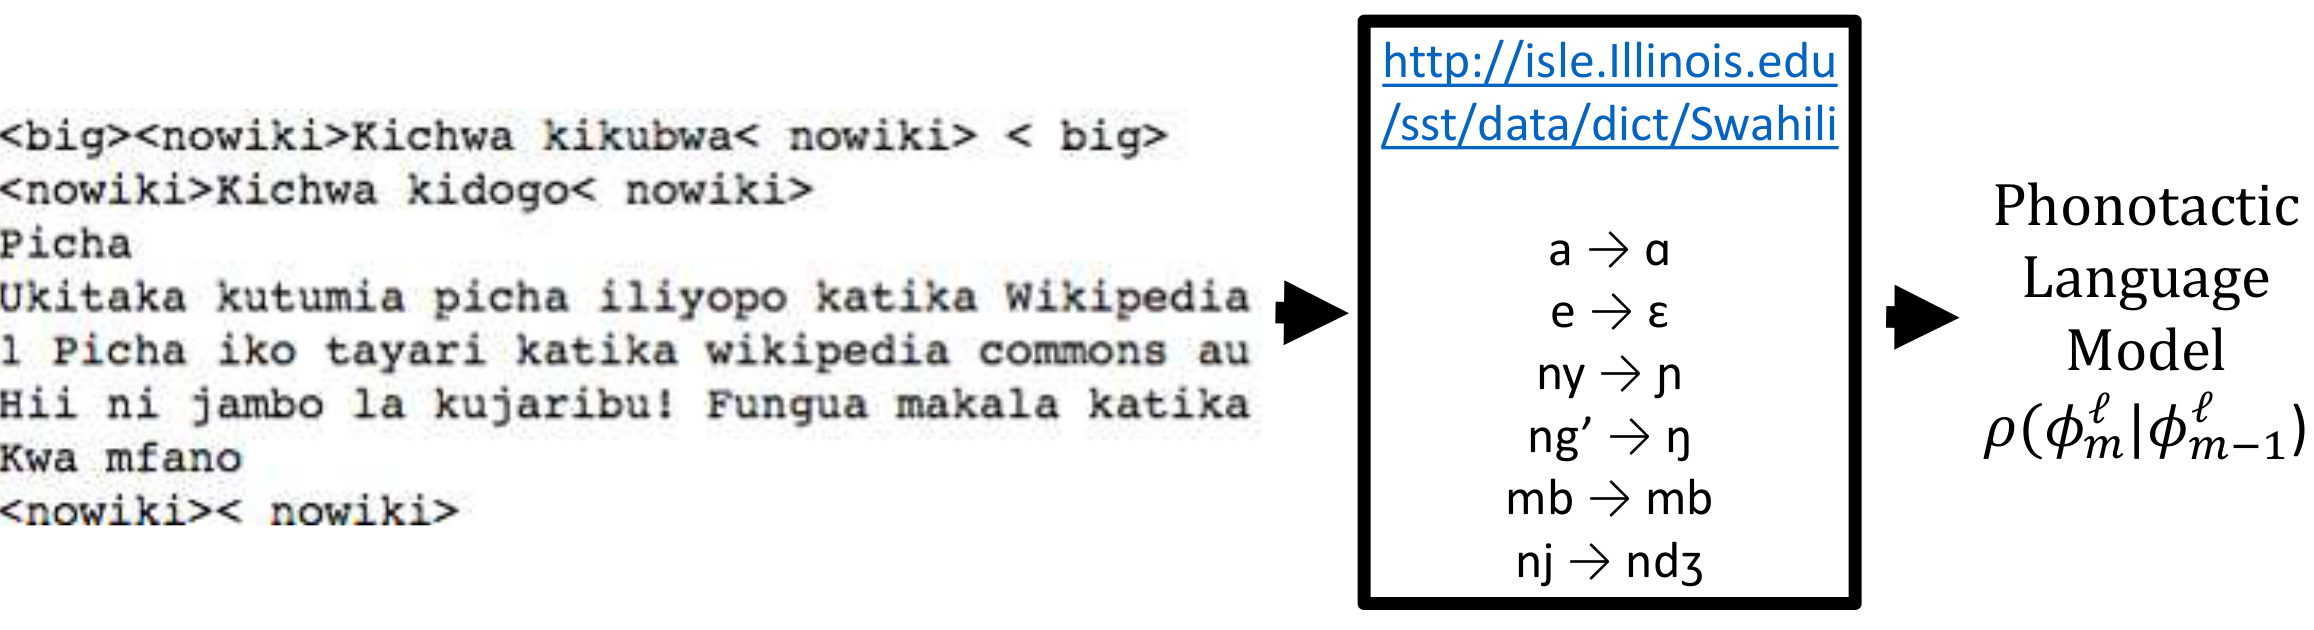
\includegraphics[width=5in]{../figs/fig_sloan.png}}
  \caption{A phonotactic language model (a bigram language model over
    phone sequences) can be trained using text data downloaded from
    Wikipedia (left), then converted into phone strings in the target
    language using a simple character-based grapheme-to-phoneme
    transducer (center).  In this example, the target language is
    Swahili.}
  \label{fig:wikitext}
\end{figure}

Fig.~\ref{fig:wikitext} shows text data downloaded from wikipedia in
Swahili, and a segment of a rule-based, character-by-character G2P for
the Swahili language~\cite{Hasegawajohnson15}.  By passing the former
through the latter, it is possible to generate synthetic phoneme
sequences in the target language.

\begin{figure}
  \centerline{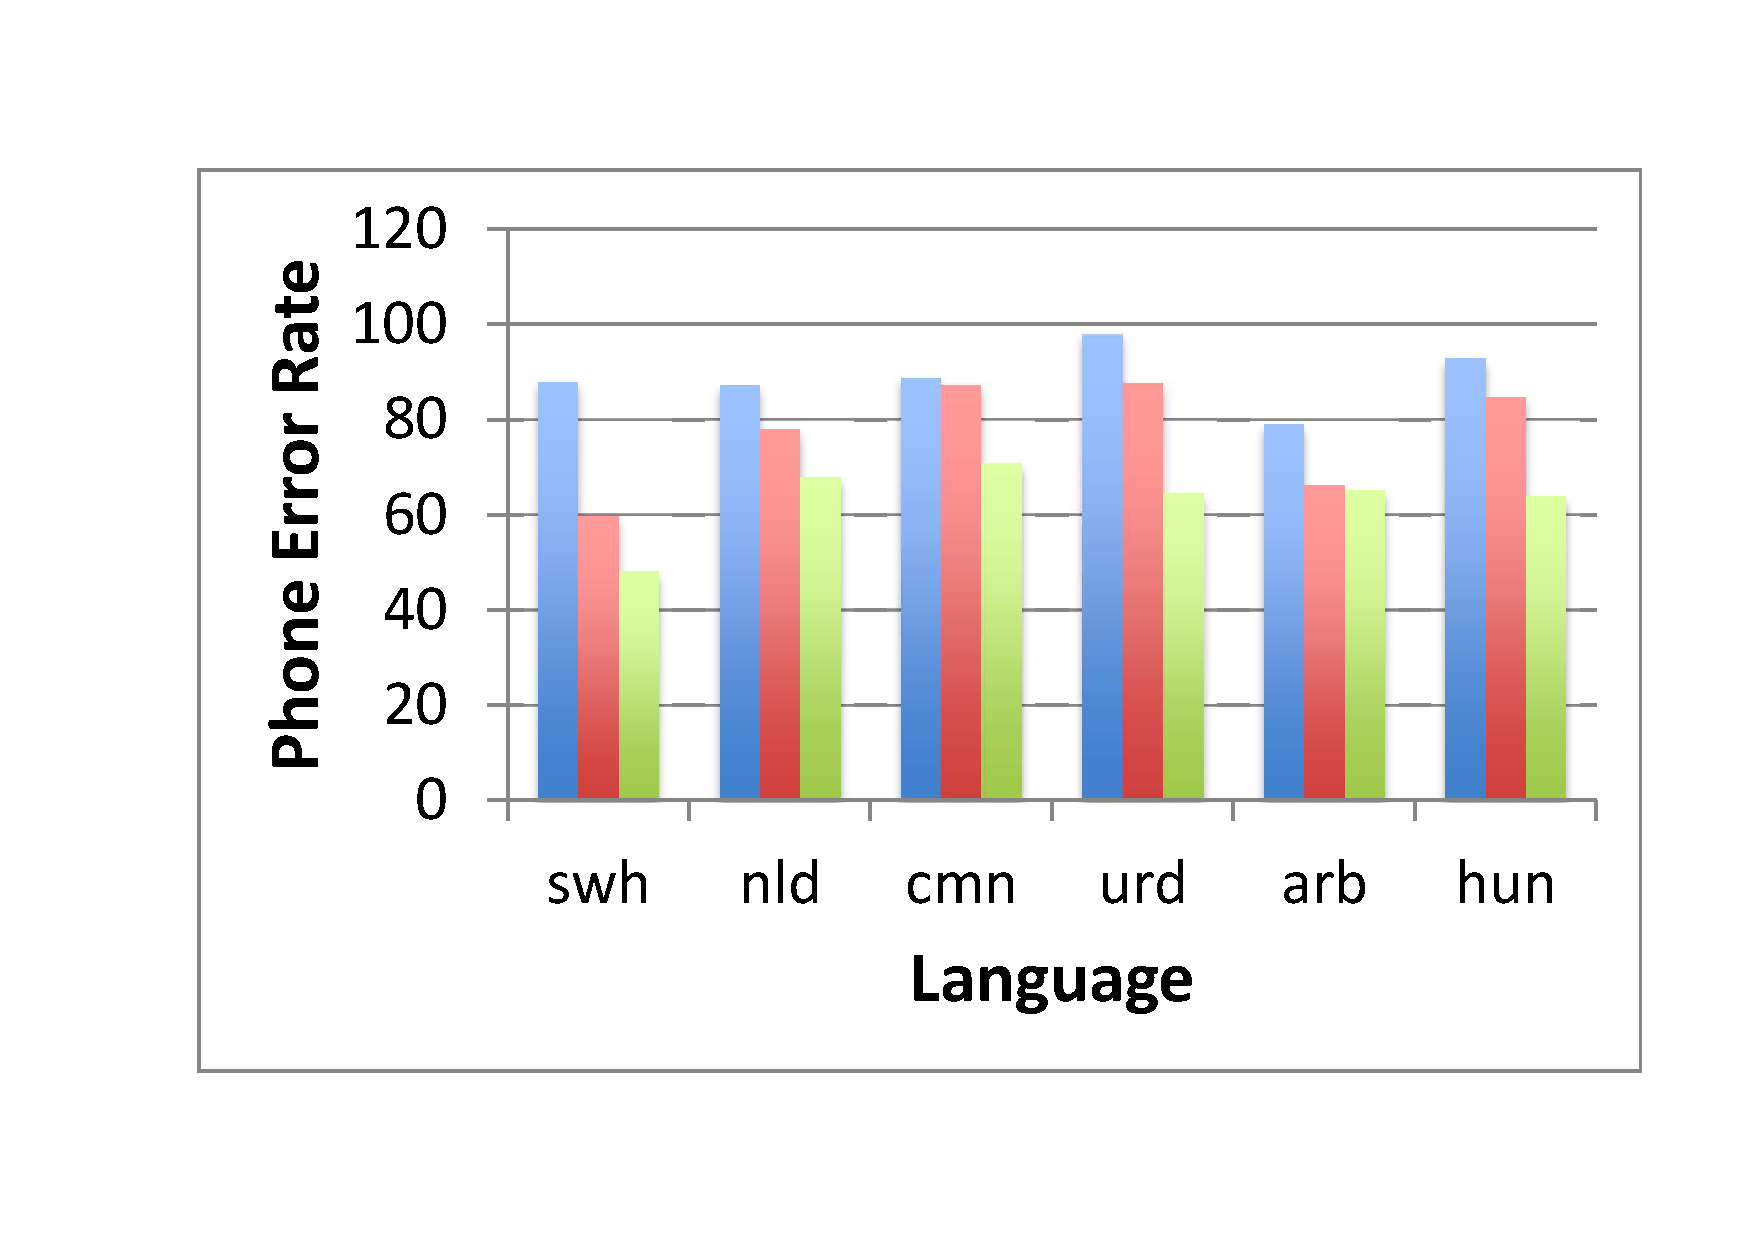
\includegraphics[width=4in]{../figs/lm_results.pdf}}
  \caption{PER of the 1-best path: a measure of the quality of
    probabilistic transcriptions acquired from mismatched
    crowdsourcing.  Native transcriptions were available in six
    languages: Swahili (SW), Dutch (DT), Mandarin (MN), Urdu (UR),
    Arabic (AR), and Hungarian (HG).  Probabilistic transcriptions
    were decoded using three different methods per language: using a
    universal phoneme set (tallest bar in each language), using a
    phoneme set specific to the target language (middle bar in each
    language), and using a phonotactic language model derived from
    wikipedia texts (shortest bar in each language).}
  \label{fig:pt_decode_per}
\end{figure}

Phone error rate of the 1-best path through the mismatched
crwodsourcing confusion network are shown in
Fig.~\ref{fig:pt_decode_per}.  As shown, the use of a phonotactic
language model, derived from wikipedia text, reduced phone error rate
by about 10\% absolute, in each language.

Composing $\mathbf{PT}\circ \mathbf{G}$ is complicated, however, by
the presence of null transitions in the PT.  A null transition in
the PT matches a non-event in the language model, for which normal
FST notation has no representation. In order to compose the PT with
the language model, therefore, it is necessary to introduce a
special type of ``non-event'' symbol, here denoted ``\#2'', into the
language model (Fig.~\ref{fig:liu1}).  As shown in
Fig.~\ref{fig:liu1}, a language model ``non-event'' is a transition
that leaves any state, and returns to the same state (a self-loop).
Such self-loops, labeled with the special symbol ``\#2'' on both
input and output language, are added to every state in the
phonotactic language model (left-hand side of Fig.~\ref{fig:liu1}).
The probabilistic transcript, then, is augmented with the special
symbol ``\#2'' as the input-language symbol for every null-output
edge
 (output symbol is $\phi_m^\ell =\epsilon$).
\begin{figure}
  \centerline{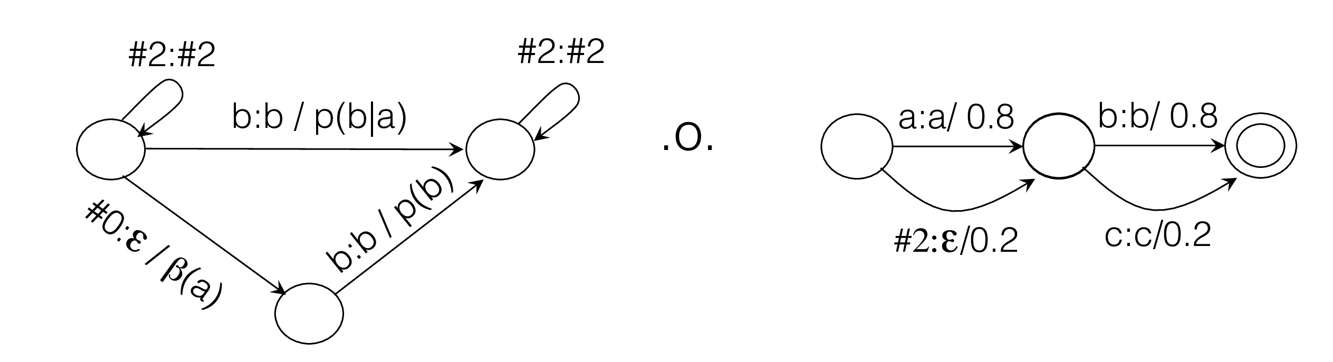
\includegraphics[width=5in]{../figs/liu1.png}}
  \caption{Deletion edges in the probabilistic transcript (edges with
    the special null output symbol, $\epsilon$), required special
    handling in order to use information from a phonotactic language
    model.  As shown, a new type of null symbol, ``\#2'', was invented
    to represent the input for every PT edge with an $\epsilon$ output
    (right).  Such edges were only allowed to match with state
    self-loops, newly added to the language model (left) in order to
    consume such non-events in the transcript.}
  \label{fig:liu1}
\end{figure}



\subsection{Maximum {\em A Posteriori} Adaptation}
\label{sec:adaptation}

Our ASR framework is based on weighted finite-state transducers (WFSTs) as outlined in~\cite{mohri2008speech}. 
In this framework, the acoustic model is specified by a probabilistic mapping from acoustic signals to a sequence of discrete symbols, and a WFST $H$ mapping these symbol sequences to triphone sequences. The other WFSTs in the framework are $C$ which maps down triphone sequences to monophone sequences, a pronunciation model $L$ and a language model $G$. Since our tasks involve phone recognition, $L$ is essentially an identity mapping and $G$ is a phone N-gram model. 

To describe the adaptation process, it will be helpful to compare the following two cases.
\begin{itemize}
\item In training the parameters of the baseline acoustic model, for each training utterance, we work with the cascade $H \circ C \circ L \circ T$, where $T$ is a linear chain FST representing the training transcript. The multilingual baselines described in Section~\ref{sec:mlbaseline} are trained in this manner using training data from languages other than the target language.

  Here, the parameters are updated using Viterbi training which computes maximum likelihood estimates based on the best path through the cascade.

\item During adaptation, for each training utterance (in the target language), we work with the cascade $H \circ C \circ L \circ PT$, where $PT$ is a WFST representing the probabilistic transcript, obtained as in Section~\ref{sec:MC}.

Here, we use maximum a posteriori (MAP) estimation to update the parameters. Further, as explained below, a lattice derived from the cascade is used instead of a single path.
\end{itemize}

%% wrong figure reference?  Shouldn't this be fig:pt ?
As noted in Figure~\ref{fig:listPER}, a PT contains significant amount of information beyond any single transcript extracted from the PT. Motivated by this, the statistics for the MAP estimation are accumulated from a lattice derived from the cascade $H \circ C \circ L \circ PT$, rather than reducing the PT to its single best path.

Though it is disadvantageous to reduce a PT to its best path, it is
nevertheless advantageous to incorporate as much information as
possible from the language model during adaptation.  Composing $L\circ
PT$ is complicated, however, by the presence of null transitions in
the PT.  A null transition in the PT matches a non-event in the
language model, for which normal FST notation has no representation.
In order to compose the PT with the language model, therefore, it is
necessary to introduce a special type of ``non-event'' symbol, here
denoted ``\#2'', into the language model (Fig.~\ref{fig:liu1}).  As
shown in Fig.~\ref{fig:liu1}, a language model ``non-event'' is a
transition that leaves any state, and returns to the same state (a
self-loop).  Such self-loops, labeled with the special symbol ``\#2''
on both input and output language, are added to every state in the
phonotactic language model (left-hand side of Fig.~\ref{fig:liu1}).
The probabilistic transcript, then, is augmented with the special
symbol ``\#2'' as the input-language symbol for every null-output edge
(output symbol is $\phi_m^\ell =\epsilon$).

\begin{figure}
  \centerline{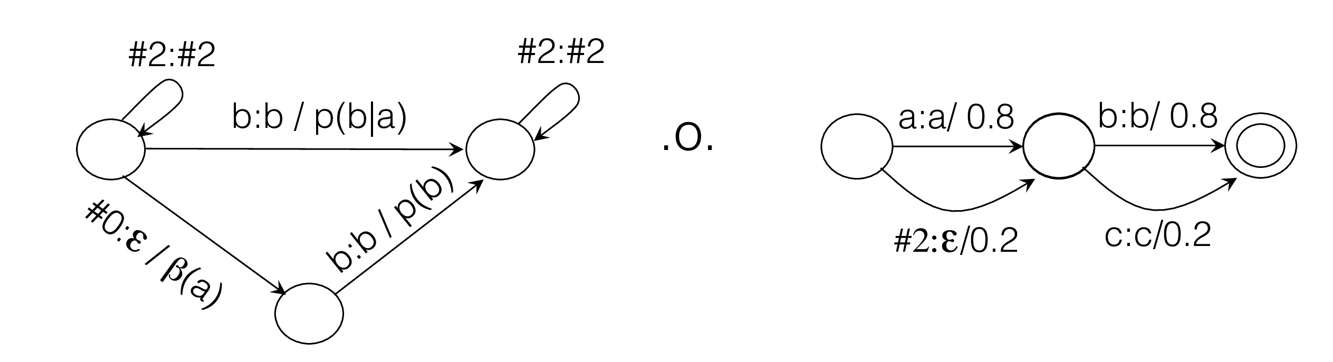
\includegraphics[width=5in]{../figs/liu1.png}}
  \caption{Deletion edges in the probabilistic transcript (edges with
    the special null output symbol, $\epsilon$), required special
    handling in order to use information from a phonotactic language
    model.  As shown, a new type of null symbol, ``\#2'', was invented
    to represent the input for every PT edge with an $\epsilon$ output
    (right).  Such edges were only allowed to match with state
    self-loops, newly added to the language model (left) in order to
    consume such non-events in the transcript.}
  \label{fig:liu1}
\end{figure}

The Bayesian framework for maximum {\em a posteriori} (MAP) estimation has
been widely applied to GMM and HMM parameter estimation problems such
as parameter smoothing and speaker
adaptation~\cite{gauvain1994maximum}.
%% single-sentence paragraph. consider merging with following paragraph.

Formally, for an unseen target language, we denote its acoustic observations $\mathbf{x}= ( x_1, \ldots, x_{T} )$, and its acoustic model parameter set as $\lambda$, then the MAP parameters are defined as:
%
\begin{equation}
  %\begin{split}
    \lambda_{\mathrm{MAP}}  = \argmax_{\lambda} \Pr(\lambda | \mathbf{x}) 
= \argmax_{\lambda} \Pr( \mathbf{x} | \lambda ) \Pr(\lambda)
%\end{split}
\label{eq:map}
\end{equation}
%
\noindent where we use multilingual baseline GMM-HMM parameters to assign the conjugate prior hyperparameters in $\rho(\lambda)$, and take the modes of the prior distributions as the initial model parameter estimates. Using suitable models for these distributions,  \cite{gauvain1994maximum} derive update rules in an EM algorithm for computing $\lambda_{\mathrm{MAP}}$. For example, the mean $\mu_{ik}$ of the GMM mixture component $k$ associated with HMM state $i$ is updated as:
\begin{align}
\tilde{\mu}_{ik} &= \frac{\tau_{ik} \mu_{ik} + \alpha_{ik} \hat{\mu}_{ik} }{\tau_{ik}  + \alpha_{ik}  } \\
\alpha_{ik}= \sum_{t=1}^{T} c_{ikt}  &\qquad\qquad\qquad
\hat{\mu}_{ik} = \frac{ \sum_{t=1}^{T} c_{ikt} x_t }{ \sum_{t=1}^{T} c_{ikt}  } \notag
\end{align}
where $\tau_{ik}$ is a hyperparameter in the prior density for the mixture component $k$ of state $i$  and $c_{ikt}$ denotes the probability of the HMM being in state $i$ with mixture component $k$ given observation $x_t$ (estimated using statistics accumulated from the cascade $H \circ C \circ L \circ PT$).  Here, $\hat{\mu}_{ik}$ is the maximum likelihood estimate of $\mu_{ik}$ given the target language data $\mathbf{x}$ and the model parameters $c_{ikt}$. Note that at each step of the iteration, $\tilde{\mu}_{ik}$ linearly interpolates between $\mu_{ik}$ and $\hat\mu_{ik}$.
In our setting,  the initial value of $\mu_{ik}$ is obtained from the multilingual baseline model, and $\tilde{\mu}_{ik}$ eventually converges to a model for the target language data.

The baseline and the adapted models were implemented using Kaldi~\cite{Kaldi2011}. In order to efficiently carry out the required operations on the cascade $H \circ C \circ L \circ PT$, we carefully designed $PT$ as an acceptor defined as $\mathrm{proj}_{\mathrm{input}} (\widehat{PT})$, where $\widehat{PT}$ is a WFST mapping phone sequences to English letter sequences obtained as a cascade of WFSTs modeling the distributions shown in Equation~\ref{eq:PT}, and $\mathrm{proj}_{\mathrm{input}}$ refers to projecting onto the input labels. For the purposes of computational efficiency, the cascade for $\widehat{PT}$ includes an additional WFST restricting the number of consecutive deletions of phones and insertions of letters (to a maximum of 3 in our experiments). We use two additional disambiguation symbols~\cite{mohri2008speech}, apart from the ones used in typical Kaldi recipes, to determinize these insertions and deletions in $\widehat{PT}$. MAP adaptation for the acoustic model was carried out for a number of iterations (12 for CA \& MD, 14 for HG \& SW, with a re-alignment stage in iteration 10).
%% This is the first mention of the particular training languages used
%% in these experiments.  I think there is need for a short section that
%% comes between sections 2 and 3 that explains the big picture of what
%% was done, in broad strokes, before getting into the mathematical
%% details of how the system was designed. Perhaps under the heading of
%% "Overview of experimental procedures" or similar.
%% 
%% Second comment: these abbreviations for languages have not been
%% introduced yet. Moreover, an international standard exists for
%% abbreviating language names (the ISO 639-3 standard). see here:
%% http://www-01.sil.org/iso639-3/codes.asp?order=639_3&letter=%25
%% for this particular sentence, Cantonese = yue, Mandarin = cmn,
%% Hungarian = hun, and Swahili = swh
%%
%% That said, I'm not sure that this point in the manuscript is the right
%% place for this particular detail of the implementation (how many
%% iterations were done for each training language). So far the rest of
%% section 3 has been about fundamental system design details that are
%% unrelated to the particular choice of training languages. I suggest
%% moving this detail to the "Experimental Methods" section. Here it
%% could just say "A variable number of iterations of the MAP adaptation
%% were carried out for the various training languages (see Section XXX 
%% for details)."


\subsection{Neural Networks}

The NN acoustic model is
\[
\pi(x_t^\ell|s_t^\ell =j,\phi^\ell,\theta)\propto
y_t^\ell(j)=\frac{1}{c_j}\frac{\exp\left(w_j^Th_t(x,\theta_h)\right)}
{\sum_k \exp\left(w_k^Th_t(x,\theta_h)\right)}
\]
whose parameters $\theta=\left\{c_j,w_j,\theta_h\right\}$ include the
senone priors $c_j$, the softmax weight vectors $w_j$, and the
parameters defining the hidden nodes $h_t(x,\theta_j)$.  NNs are
trained by using a GMM-HMM to compute an initial senone posterior,
$\pi(s_t^\ell=j,x^\ell|\theta)$, then minimizing the cross-entropy
between the estimated senone posterior and the neural network output
$y_{t}^\ell(j)$,
%.  The cross entropy is measured as
%\begin{equation}
%  H(S^\ell\Vert Y^\ell)=-\sum_{t=1}^T \sum_{j} \pi(s_t^\ell=j) \ln y_{t}^\ell(j)
%  \label{eq:dnn_train}
%\end{equation}
%The gradient of Eq.~(\ref{eq:dnn_train}) with respect to its model
%parameters is
using gradient descent in the direction
\begin{equation}
  -\nabla_\theta H(S^\ell\Vert Y^\ell)=
  \sum_{t=1}^T\sum_j\frac{\pi(j,x^\ell|\theta)}{y_t^\ell(j)}
  \nabla_\theta y_t^\ell(j)
  \label{eq:dnn_dt}
\end{equation}
NN training with deterministic transcriptions is improved by
quantizing $\pi(s_t^\ell,x^\ell|\theta)\rightarrow\left\{0,1\right\}$
using forced alignment~\cite{Morgan95}. Preliminary experiments showed
that forced alignment also improves the accuracy of NNs trained from
probabilistic transcriptions: the best path through the PT, and the
best alignment of the resulting senones to the waveform, were both
computed using forced alignment.  The resulting best senone string was
used to train a NN using Eq.~(\ref{eq:dnn_dt}).



%%%%%%%%%%%%%%%%%%%%%%%%%%%%%%%%%%%%%%%%%%%%%%%%
\section{Experimental Methods}
\label{sec:methods}

Our goal is to train a phone recognition system for a given target
language in which no native transcriptions are available. We assume
that we have access to unspoken texts and to untranscribed audio in
the target language, but not to transcribed audio
(Sec.~\ref{sec:data}).  Mismatched crowdsourcing was interpreted using
a multilingual misperception G2P (Sec.~\ref{sec:methodsmc}), or using
a language-specific misperception G2P estimated using EEG
(Sec.~\ref{sec:methods_eeg}).  Baseline multilingual systems are
trained using native transcriptions from several different languages
not including the target language (Section~\ref{sec:mlbaseline}).
Finally, parameters of the acoustic model are adapted using PTs in the
target language, derived from either self-training or from mismatched
transcriptions (Sec.~\ref{sec:ptadapt}).


\subsection{Data}
\label{sec:data}

Speech data were extracted from publicly available podcasts~\cite{SBS}
hosted in 68 different languages.  In order to generate test corpora
(in which it is possible to measure phone error rate), advertisements
were posted at the University of Illinois seeking native speakers
willing to transcribe speech in any of these 68 languages.  Of the ten
transcribers who responded, six people were each able to complete one
hour of speech transcription (the other four dropped out).  One
additional language was transcribed by workers recruited at $I^2R$ in
Singapore, yielding a total of seven languages with native
transcriptions suitable for testing an ASR: Arabic (arb), Cantonese
(yue), Dutch (nld), Hungarian (hun), Mandarin (cmn), Swahili (swh) and
Urdu (urd).

The podcasts were not entirely homogeneous in the target
language and contain utterances interspersed with segments of music
and English. A simple GMM-based language identification system was
developed as a first pass over the podcasts in order to isolate
regions that correspond mostly to the target language. These long
segments were then split into smaller $\approx$ 5-second
segments. This was to enable easy labeling by the native transcribers,
and more importantly to allow for the collection of mismatched
transcriptions that required the speech segments to be short. To
further check that only speech clips in the target language were
retained, the native transcribers were asked to omit any 5-second
clips that contained music, significant amounts of noise, English
speech or speech from multiple speakers. The resulting transcribed
speech clips roughly amounted to 45 minutes of speech in Urdu and 1
hour of speech in the remaining six languages. The orthographic
transcriptions for these clips were then converted into phonemic
transcriptions using language-specific dictionaries and G2P mappings
(these resources are detailed in Section~\ref{sec:mlbaseline}). For
each language, we chose a random 40/10/10 minutes split into training,
development and evaluation sets.  Table~\ref{tab:data} describes the
resulting training, development and evaluation sets.
\begin{table}[t]
\centering
\begin{tabular}{|c||c|c|c|c|c|c|c|}\hline
Speech  & \multicolumn{7}{c|}{Language Code (ISO 639-3)}\\\hline
(\# phones) & arb & yue & nld & hun & cmn & swh & urd \\ \hline\hline
Train & 32486 & 32693 & 27314 & 29461 & 28571 & 30009 & 21275 \\
Dev & 8208 & 6860 & 6943 & 7873 & 8244 & 7658 & 5808 \\
Eval & 8191 & 8638 & 6582 & 7474 & 7035 & 7441 & 3689 \\\hline
\end{tabular}
\caption{Data statistics for seven podcast languages listing number of
phones in the training/development/evaluation sets.}
\label{tab:data}
\end{table}

\subsection{Mismatched Crowdsourcing}
\label{sec:methodsmc}

Mismatched transcripts were collected from crowd workers (Turkers)
on Amazon Mechanical Turk.
%for all the data listed in
%Table~\ref{tab:data}.  The crowdsourcing task setup is described
%in~\cite{JHJ15b}.
Each 5-sec speech segment was further split into 4
non-overlapping segments to make the non-native listening task
easier. The crowdsourcing task was set up as described
in~\cite{JHJ15b}; briefly, the segments were played to Turkers,
who transcribed what they heard (typically in the form of nonsense
syllables) using English orthography. Each segment was
transcribed by 10 distinct Turkers. More than 2500 Turkers
participated in these tasks, with roughly 30\% of them claiming to
know only English (Spanish, French, German, Japanese, Chinese were
some of the other languages listed by the Turkers).


\subsection{Channel Model from EEG}

EEG signals were acquired, and used to estimate a mismatch model of
the form shown in Eqs.~\ref{eq:dfdist} and~\ref{eq:eegdist}.  All
methods were approved by the University of Washington Institutional
Review Board.

In the finite duration of an EEG experiment, it is not possible to ask
human subjects to listen to sounds from many languages.  Two languages
other than English were chosen: one language judged to be similar to
English, one judged to be maximally different.  Inter-language
similarity was estimated based on the frequency of many-to-one
mappings ($N_{M2O}(\mathbb{\Phi})$) between the English phoneme
inventory ($\mathbb{\Psi}$) and the phoneme inventory
$\mathbb{\Phi}$. This quantity was defined by finding, for each
non-native phoneme $\phi$, the English phoneme $\psi^*(\phi)$ to which
it is most similar:
\begin{equation}
  \psi^*(\phi) = \argmin \sum_k \delta\left(f_k(\psi)\ne f_k(\phi)\right)
\end{equation}
The number of many-to-one collisions is then defined as
\begin{equation}
  N_{M2O}(\mathbb{\Phi})=\frac{1}{|\mathbb{\Psi}|}\sum_{\phi_1\ne\phi_2}
  \delta\left(\psi^*(\phi_1)=\psi^*(\phi_2)\right)
\label{eq:m2o}
\end{equation}
where $|\mathbb{\Psi}|$ is the size of the English phoneme inventory.
The frequency of many-to-one collisions is listed in
Table~\ref{tab:m2o} for several languages.  By this metric, Hindi
(HIN) is the language most dissimilar from English.  Spanish (SPA) is
the language most similar to English, followed by Portuguese (POR) and
Dutch (NLD).  Spanish is heard frequently on television in the United
States, so in order to avoid using a language with which listeners
have excessive familiarity, Dutch was selected as a representative of
the set of languages similar to English.

\begin{table}
  \centerline{\begin{tabular}{|lr|lr|lr|}\hline
    $\mathbb{\Phi}$ & $N_{M2O}(\mathbb{\Phi})$ & 
    $\mathbb{\Phi}$ & $N_{M2O}(\mathbb{\Phi})$ & 
    $\mathbb{\Phi}$ & $N_{M2O}(\mathbb{\Phi})$ \\ \hline
    SPA & 0.862 & YUE & 1.280 & CMN & 1.531 \\
    POR & 1.152 & JPN & 1.333 & AMH & 1.844 \\
    NLD & 1.182 & VIE & 1.393 & HUN & 1.857 \\
    DEU & 1.258 & KOR & 1.429 & HIN & 2.848 \\\hline
  \end{tabular}}
  \caption{Frequency of many-to-one mappings $N_{M2O}(\mathbb{\Phi})$
    between phoneme inventory $\mathbb{\Phi}$ and the inventory of
    English.  Languages listed by ISO 639-3 codes.}
  \label{tab:m2o}
\end{table}

Eighteen consonants and two vowels were selected from the phoneme
inventory of each language, then two native speakers of Dutch and two
of Hindi (one male and one female in each language) recorded
consonant-vowel syllables spanning the 56 possible combinations in
each language.  Recorded syllables had an average duration of 400ms,
and were presented with an inter-stimulus interval of 350ms to
headphones worn by one speaker of American English.  An EEG recording
cap was used to acquire electrocortical responses of the subject in
response to each stimulus.

Since EEG signals were only acquired in response to two distinct
vowels, it was not possible, using these training data, to learn
classifiers that distinguish vowels.  Classifiers were trained for
most of the consonantal distinctive features of English, but not all.
Fig.~\ref{fig:eeg_svm_eers} shows equal error rates of these
classifiers when applied to English consonants, and when applied
(without re-training) to Dutch or Hindi consonants.

\begin{figure}
  \centerline{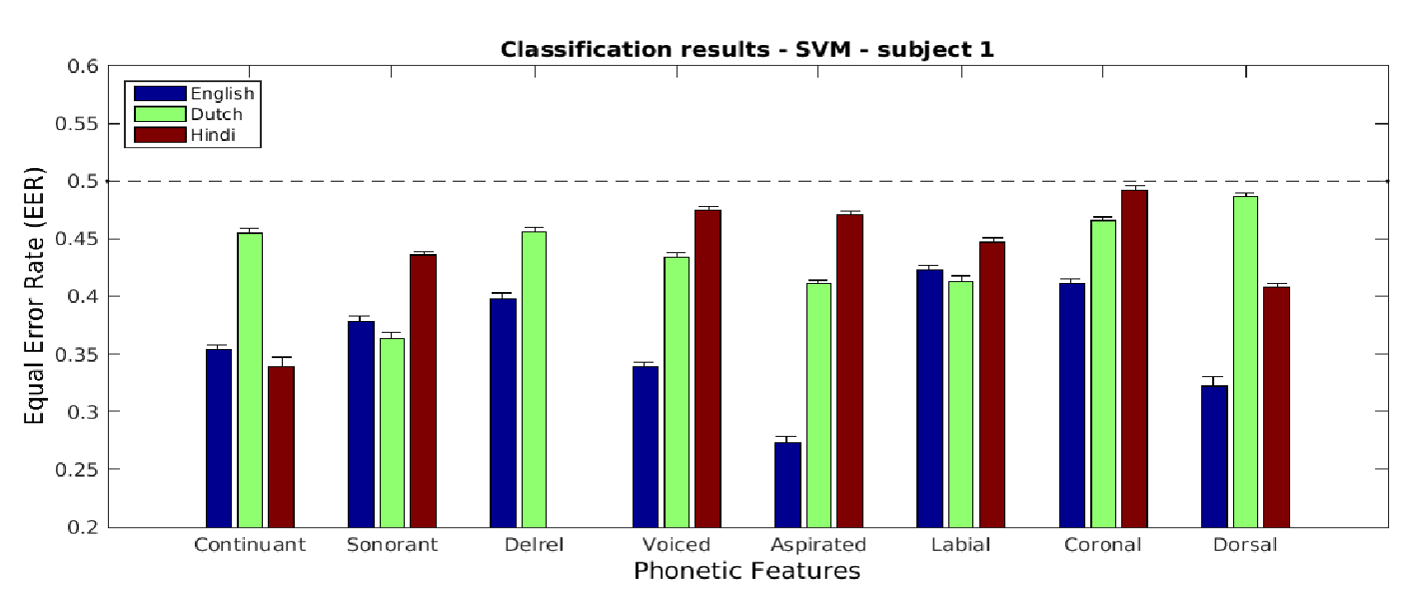
\includegraphics[width=5in]{../figs/diliberto_svmresults.png}}
  \caption{Classifiers were trained to observe EEG signals, and to
    classify the distinctive features of the phoneme being audited.
    Equal error rates are shown for English (the language used in
    training; train and test data did not overlap), Dutch, and Hindi
    (not used in training).}
  \label{fig:eeg_svm_eers}
\end{figure}

Eqs.~\ref{eq:dfdist} defines a log-linear model of $\rho(\psi|\phi)$, the
probability that Dutch phoneme $\phi$ will be perceived as English
phoneme $\psi$.  Denote by $\rho_U(\psi|\phi)$ the model of
Eq.~\ref{eq:dfdist} with uniform weights for all distinctive features
($w_k=\alpha$, a tunable constant).  Denote by $\rho_{EEG}(\psi|\phi)$ the
same model, but with weights $w_k$ derived from EEG measurements
(Eq.~\ref{eq:eegdist}).  Fig.~\ref{fig:eeg_confusions} shows these
two confusion matrices: $\rho_U(\psi|\phi)$ on the left,
$\rho_{EEG}(\psi|\phi)$ on the right.  The figure clearly shows the
difference between these two distributions.  The entropy of the
uniform distribution, $\rho_U(\psi|\phi)$, is too low: when a Dutch
phoneme $\phi$ has a nearest-neighbor $\psi^*(\phi)$ in English, then
few other phonemes are considered to be possible confusions.
$\rho_{EEG}(\psi|\phi)$ has a very different problem: since distinctive
feature classfiers have been trained for only a small set of
distinctive features (in particular, no vowel classifiers were
trained), there are large groups of phonemes whose confusion
probabilities can not be distinguished (giving the figure its
block-diagonal structure).  The faults of both models can be
ameliorated by interpolating them in some way, e.g., by computing the
linear interpolation
$\rho_I(\psi|\phi)=a\rho_U(\psi|\phi)+(1-a)\rho_{EEG}(\psi|\phi)$ for some
constant $0\le a\le 1$.

\begin{figure}
  \centerline{
    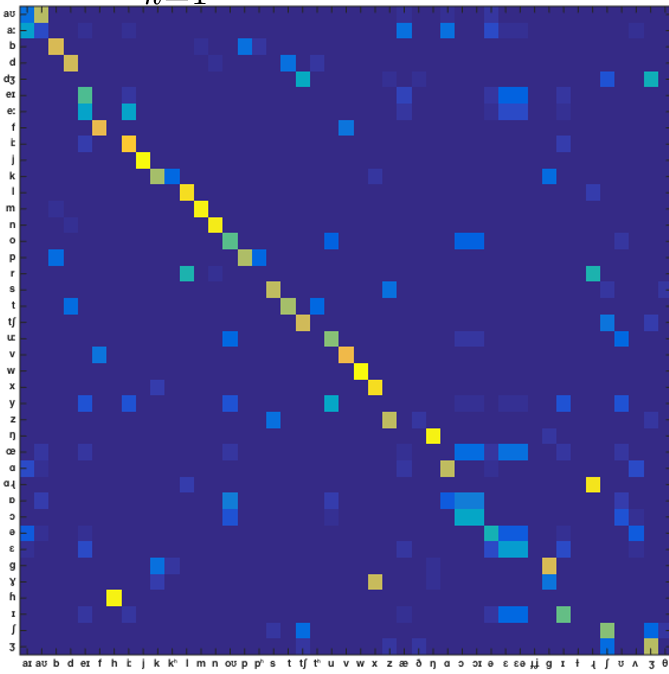
\includegraphics[width=3in]{../figs/mirbagheri_dist_features.png}
    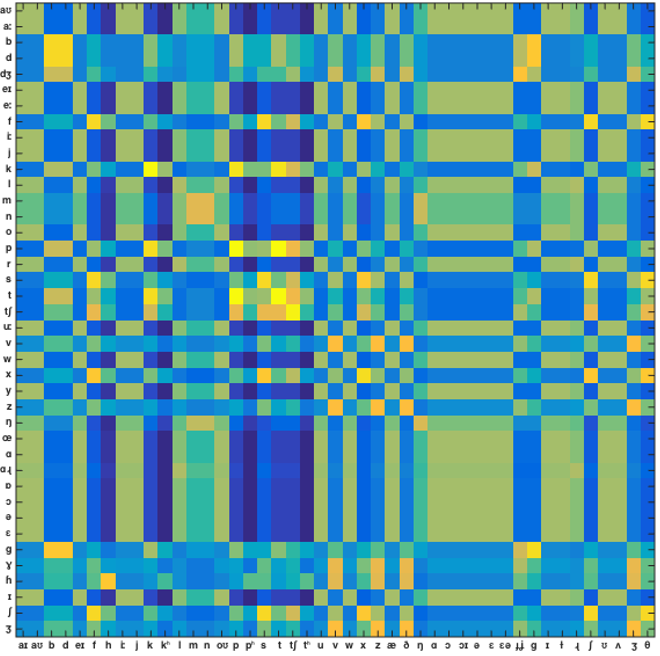
\includegraphics[width=3in]{../figs/mirbagheri_dist_eeg.png}
  }
  \caption{Phoneme confusion probabilities between English phonemes
    (column) and Dutch phonemes (row) using models in which the log
    probability is proportional to distance between the corresponding
    distinctive feature vectors.  Left: all features have the same
    weight.  Right: feature weights equal negative log error rate of
    EEG signal classifiers.}
  \label{fig:eeg_confusions}
\end{figure}
    

\subsection{Cross-Lingual Baselines}
\label{sec:mlbaseline}

The goal of building a cross-lingual system is two-fold.
One is to define a baseline for generalizing to an unseen
language without any labeled audio corpus.  The other
is have the baseline serve as a starting point for
adaptation.

The dataset consists of 40 minutes of labeled audio for training,
10 minutes for development, and 10 minutes for testing
for each language.
%The orthographic transcripts are converted into
%phonetic transcripts using language-dependent G2Ps.
%Beginning with a list of the IPA symbols used in canonical descriptions
%of all seven languages,
%any symbol appearing in only one language was merged with a different symbol
%differing by only one distinctive feature; this process proceeded until 
%each remaining phone symbol is represented in at least two languages.
English words in each transcript are identified and converted to phones with
an English G2P trained using CMUdict~\cite{Lenzo1995}, then
other words are converted into phonetic transcripts using language-dependent
dictionaries and G2Ps.
%We take the canonical pronunciation of a word if the word
%appears in a lexicon,
%otherwise estimate the word's pronunciation using a G2P.
The Arabic dictionary is from the Qatari Arabic Corpus~\cite{Elmahdy14},
the Dutch dictionary is from CELEX v2~\cite{Baayen96},
the Hungarian dictionary was provided by BUT~\cite{Grezl14},
the Cantonese dictionary is from $I^2R$,
the Mandarin dictionary is from CALLHOME~\cite{LDC96},
and the Urdu and Swahili G2Ps were compiled from
character-based descriptions of the orthographic systems in those
two languages.

Each HMM was trained with data from six languages, tuned
(stream weight and insertion penalty)
on the development set of the seventh language, and
tested on the evaluation set of the seventh language.  The lexicon of
the target language was not used during testing, but two types of
language-dependent specialization were allowed.  In the first type of
specialization, the universal phone set was restricted at test time to
output only phones in the target language.  In the second type of
specialization, a target-language phone bigram language model was
trained using phone sequences converted from Wikipedia texts.
%text.  The texts were
%collected from Wikipedia articles linked from the main page of each
%language crawled once per day over four months.
As an oracle experiment, we also train language dependent
HMMs for each individual language with 40 minutes of labeled audio.


\subsection{MAP Adaptation to Probabilistic Transcripts}
\label{sec:ptadapt}

The baseline and the adapted models were implemented using
Kaldi~\cite{Kaldi2011}. In order to efficiently carry out the required
operations on the cascade $H\circ C\circ PT\circ G$, $PT$ was defined
as $\mathrm{proj}_{\mathrm{input}} (\widehat{PT})$, where
$\widehat{PT}$ is a WFST mapping phone sequences to English letter
sequences (Eq.~\ref{eq:PT}), and $\mathrm{proj}_{\mathrm{input}}$
refers to projecting onto the input labels. For the purposes of
computational efficiency, the cascade for $\widehat{PT}$ includes an
additional WFST restricting the number of consecutive deletions of
phones and insertions of letters (to a maximum of 3). Two additional
disambiguation symbols~\cite{mohri2008speech} were used to determinize
these insertions and deletions in $\widehat{PT}$. MAP adaptation for
the acoustic model was carried out for a number of iterations (12 for
yue \& cmn, 14 for hun \& swh, with a re-alignment stage in iteration
10).


%%%%%%%%%%%%%%%%%%%%%%%%%%%%%%%%%%%%%%%%%%%%%%%%%%%%%%%%%%
\section{Experimental Results}
\label{sec:results}

This section reports two types of results.  First,
subsections~\ref{s6:mc} and~\ref{ssec:eeg} report improvements in the
quality of probabilistic transcription using information acquired from
text-based phone language models and EEG signals, respectively.
Second, subsections~\ref{s6:mlbaseline} and~\ref{ssec:asr} reports the
accuracy of cross-lingual ASR and PT-adapted ASR, respectively.


\subsection{Mismatched Crowdsourcing}
\label{s6:mc}

\begin{figure}
  \centerline{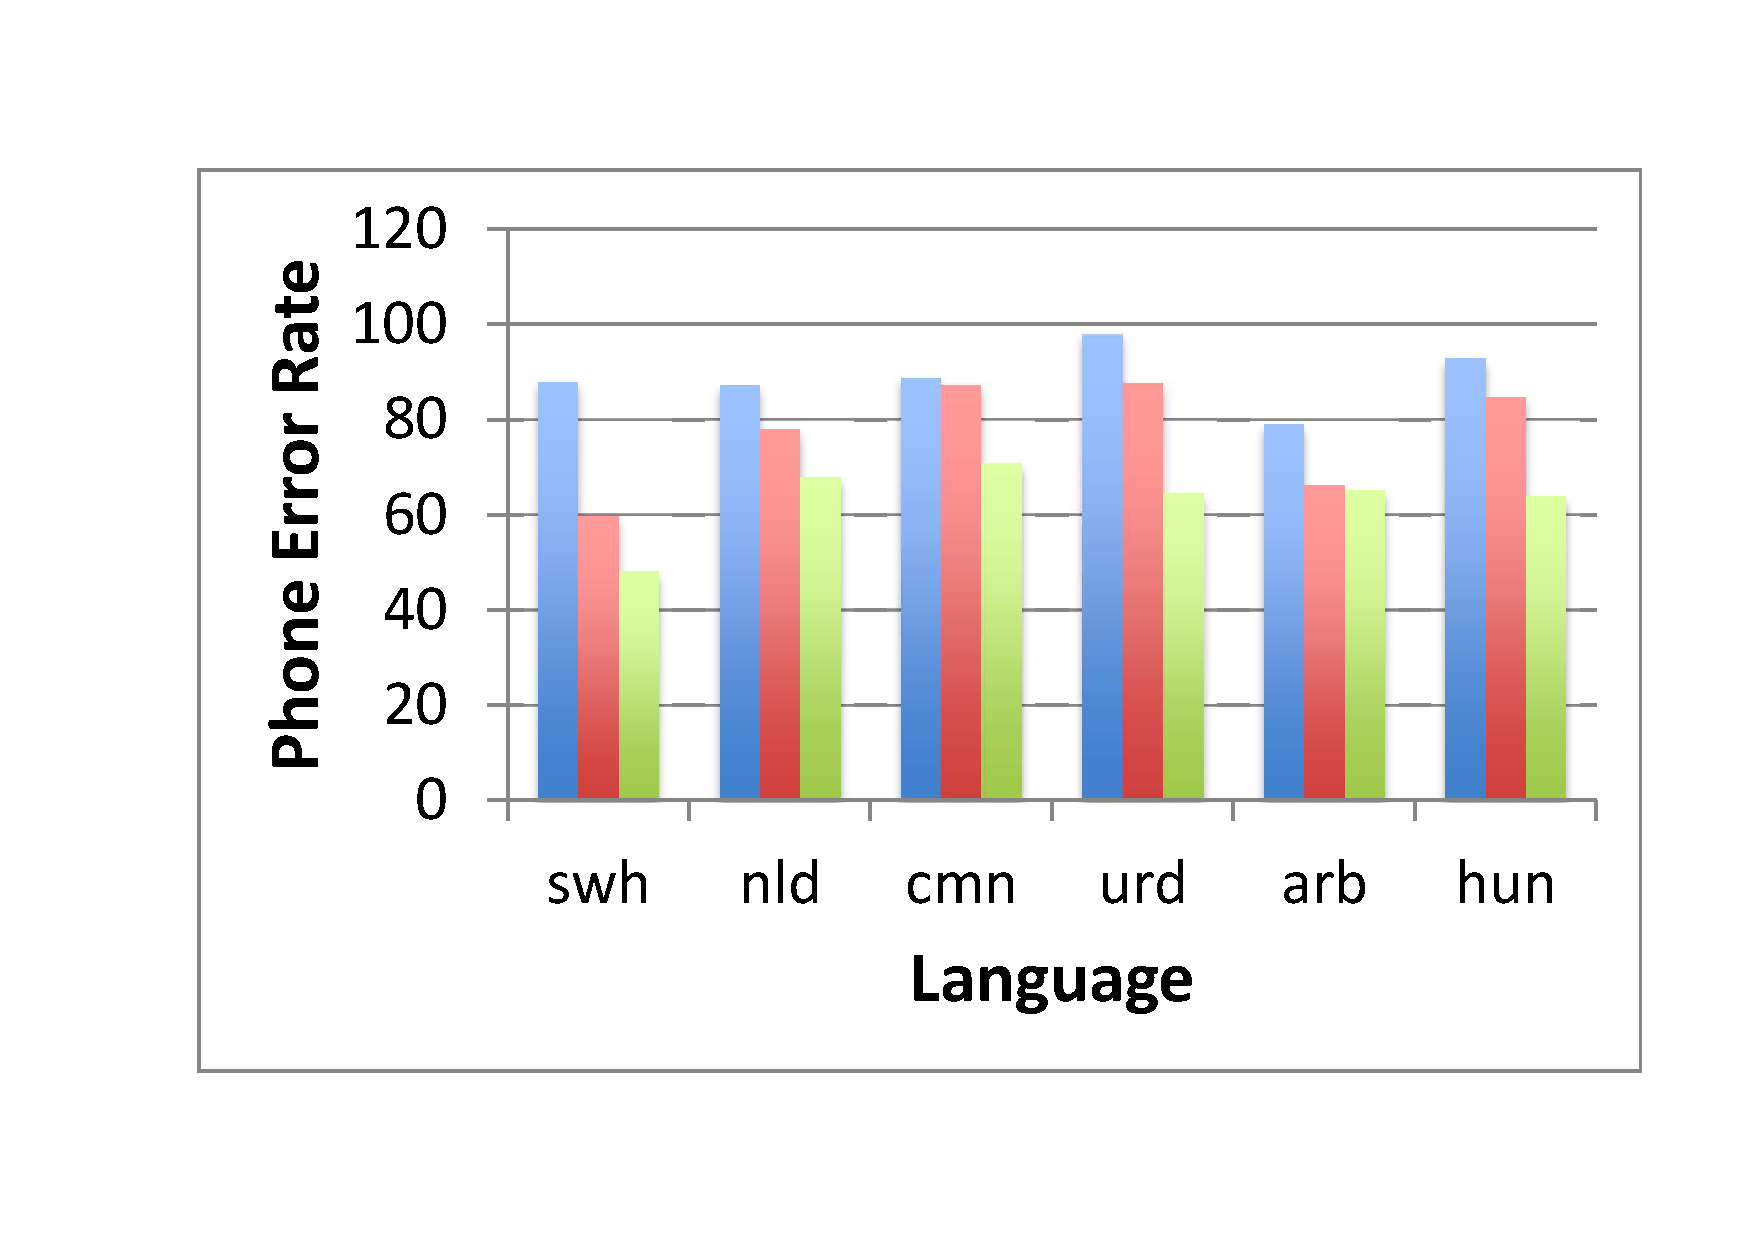
\includegraphics[width=4in]{../figs/lm_results.pdf}}
  \caption{PER of the 1-best path: a measure of the quality of
    probabilistic transcriptions acquired from mismatched
    crowdsourcing.  Native transcriptions were available in six
    languages: Swahili (swh), Dutch (nld), Mandarin (cmn), Urdu (urd),
    Arabic (arb), and Hungarian (hun).  Probabilistic transcriptions
    were decoded using three different methods per language: using a
    universal phoneme set (tallest bar in each language), using a
    phoneme set specific to the target language (middle bar in each
    language), and using a phonotactic language model derived from
    wikipedia texts (shortest bar in each language).}
  \label{fig:pt_decode_per}
\end{figure}

The quality of a probabilistic transcription derived from mismatched
crowdsourcing is significantly improved by using a phone language
model during the decoding process ($\rho(\phi)$ in Eq.~\ref{eq:PT}).
A crude measure of the quality of the PTs is given by the phone error
rate between $\phi^* = \argmax_{\phi} \rho(\phi|T)$ and the reference
phone sequences, called the ``label phone error rate'' (LPER).Phone
language models for each target language were computed from Wikipedia
texts using the methods described in Sec.~\ref{sec:trainwithlm}.
LPER of the 1-best path through the resulting PTs are shown in
Fig.~\ref{fig:pt_decode_per}.  As shown, the use of a phonotactic
language model, derived from wikipedia text, reduces PER by about 10\%
absolute, in each language.

%\begin{table}[t]
%\centering
%\begin{tabular}{|c||c|c|c|c|c|c|c|}
%  \hline
%  & \multicolumn{7}{|c|}{Language (ISO 639-3 Code)}\\ \hline
%& arb & yue & nld & hun & cmn & swh & urd \\ \hline\hline
%Dev set (1-best PER) & 65.8 & 66.4 & 68.9 & 63.7 & 70.9 & 47.6 & 67.2 \\
%Eval set (1-best PER) & 66.2 & 67.8 & 70.9 & 63.5 & 69.6 & 50.3 & 70.5 \\\hline
%\end{tabular}
%\caption{Error rates (PER) of probabilistic transcripts computed from
%  mismatched crowdsourcing (non-native human listeners): Phone error
%  rate (PER) of the 1-best path through the probabilistic
%  transcription, $\phi^*=\argmax\rho(\phi|T)$, development and
%  evaluation sets.}
%\label{tab:LPER}
%\end{table}

%Table~\ref{tab:LPER} lists LPERs on the SBS development and evaluation
%sets, for all seven languages.
LPER of the 1-best path does not
accurately reflect the extent of information in the PTs that can be
leveraged during ASR adaptation.  Consider, for example, the four
Urdu phones~\ipa{[p,p\textsuperscript{h},b,\"*b]}.  An attentive
English-speaking transcriber must choose between the two letters
$<$p,b$>$ in order to represent any of these four phones.  The
misperception G2P therefore maps the letters $<$p,b$>$ into a
distribution over the phones~\ipa{[p,p\textsuperscript{h},b,\"*b]}.
There is no reason to expect that the maximizer of
$\rho(\phi|\lambda)$ is correct, but there is good reason to expect
the correct answer to be a member of a short $N$-best list ($N\le 4$
phones/grapheme).  A fuller picture is therefore obtained by
considering a collection of sequences $\phi$ that are almost as
probable as $\phi^*$ according to our model. Figure~\ref{fig:listPER}
shows the trend of phone error rates (for three languages) obtained by
using collections $\phi$ of increasing size, plotted against an
entropy estimate of $\phi$, e.g., 1 bit of entropy allows two equally
probable choices for each phone in $\phi$. We note that the phone
error rates significantly drop across all languages, staying within 1
bit of entropy per phone, illustrating the extent of information
captured by the PTs.

\begin{figure}[t!]
\begin{center}
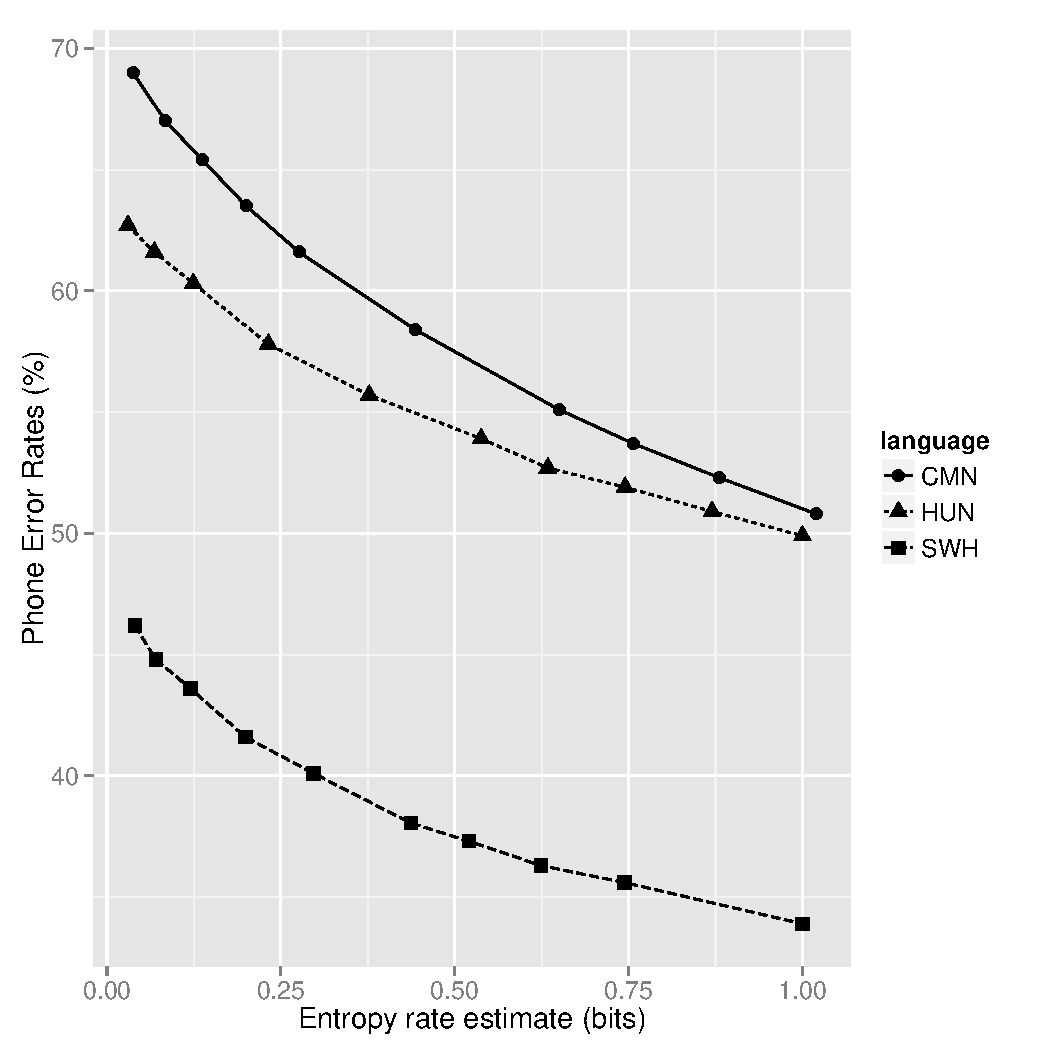
\includegraphics[width=3in]{../figs/perfig.pdf}
\end{center}
\caption{LPER plotted against entropy rate estimates of phone sequences in three different languages.}
\label{fig:listPER}
\end{figure}


\subsection{Misperception Transducer Trained Using EEG}
\label{ssec:eeg}

\newcommand{\specialcell}[2][c]{%
  \begin{tabular}[#1]{@{}c@{}}#2\end{tabular}}

Epoched and feature-coded EEG data {\em for the English syllables only}
were used to train a support vector machine classifier for each distinctive feature.
The classifiers were then used (without re-training) to classify the
EEG responses to the and Hindi syllables.
Fig.~\ref{fig:eeg_svm_eers} shows equal error rates of these
classifiers when applied to the three languages.

\begin{figure}
  \centerline{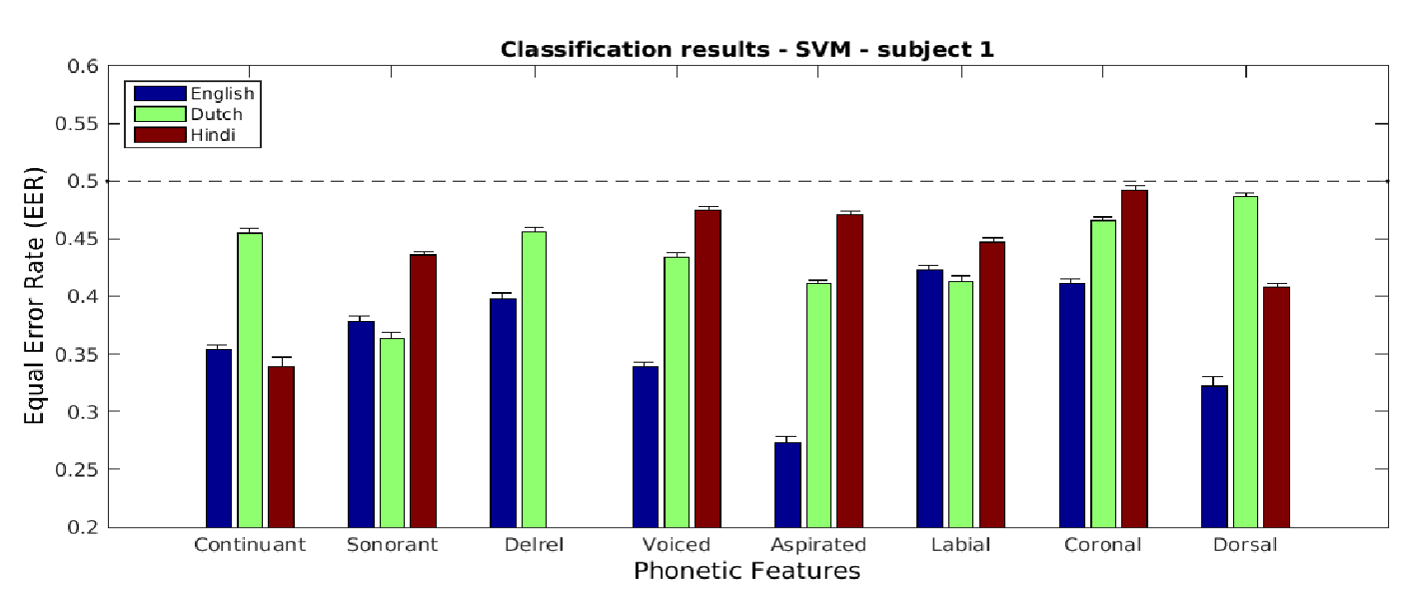
\includegraphics[width=5in]{../figs/diliberto_svmresults.png}}
  \caption{Classifiers were trained to observe EEG signals, and to
    classify the distinctive features of the phone being heard.  Equal
    error rates are shown for English (the language used in training;
    train and test data did not overlap), Dutch, and Hindi.  Dashed
    line shows chance=50\%.}
  \label{fig:eeg_svm_eers}
\end{figure}

Eq.~(\ref{eq:dfdist}) defines a log-linear model of $\rho(\psi|\phi)$,
the probability that a non-English phoneme $\phi$ will be perceived as
English phoneme $\psi$.  Denote by $\rho_U(\psi|\phi)$ the model of
Eq.~(\ref{eq:dfdist}) with uniform weights for all distinctive
features ($w_k=\alpha$, a tunable constant).  Denote by
$\rho_{EEG}(\psi|\phi)$ the same model, but with weights $w_k$ derived
from EEG measurements (Eq.~(\ref{eq:eegdist})).
Fig.~\ref{fig:eeg_confusions} shows these two confusion matrices:
$\rho_U(\psi|\phi)$ on the left, $\rho_{EEG}(\psi|\phi)$ on the
right. The entropy of the uniform weighting, $\rho_U(\psi|\phi)$, is
too low: when a Dutch phoneme $\phi$ has a nearest-neighbor
$\psi^*(\phi)$ in English, then few other phonemes are considered to
be possible confusions.  $\rho_{EEG}(\psi|\phi)$ has a very different
problem: since distinctive feature classfiers have been trained for
only a small set of distinctive features, there are large groups of
phonemes whose confusion probabilities can not be distinguished
(giving the figure its block-diagonal structure).  The faults of both
models can be ameliorated by interpolating them in some way, e.g., by
computing the linear interpolation
$\rho_I(\psi|\phi)=a\rho_U(\psi|\phi)+(1-a)\rho_{EEG}(\psi|\phi)$ for
some constant $0\le a\le 1$.

\begin{figure}
  \centerline{
    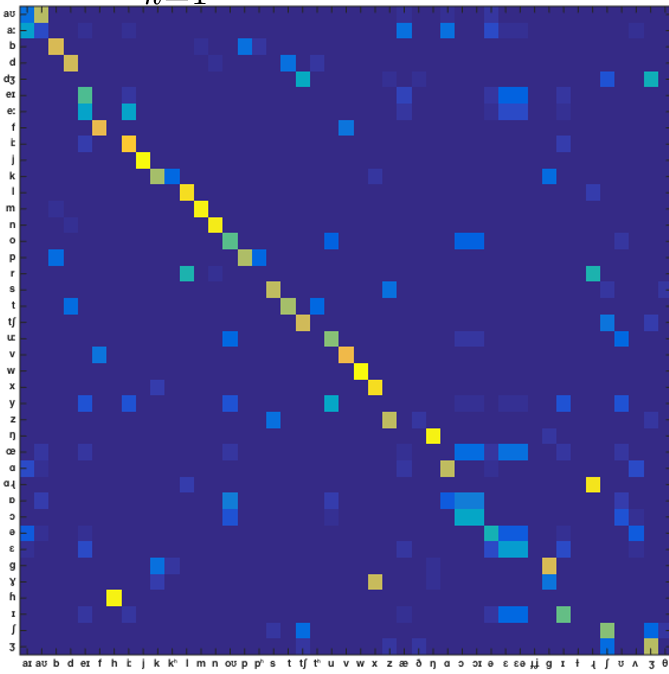
\includegraphics[width=3in]{../figs/mirbagheri_dist_features.png}
    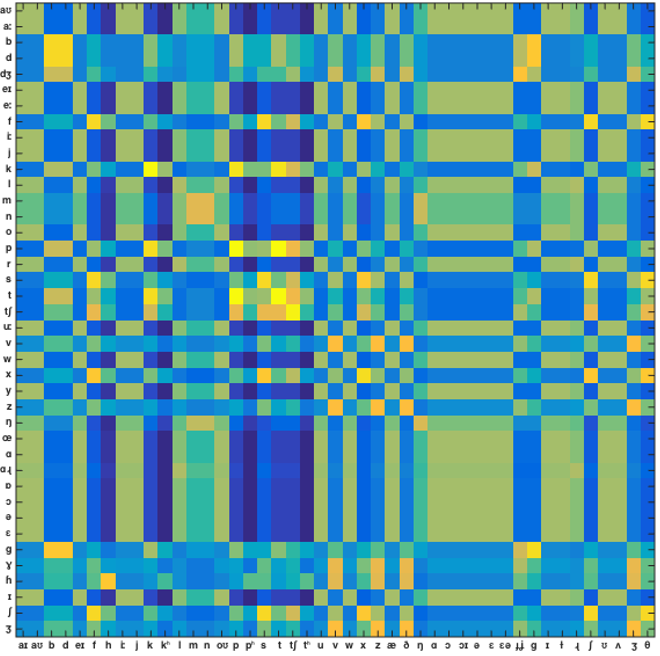
\includegraphics[width=3in]{../figs/mirbagheri_dist_eeg.png}
  }
  \caption{Phoneme confusion probabilities between English phonemes
    (column) and Dutch phonemes (row) using models in which the log
    probability is proportional to distance between the corresponding
    distinctive features.  Left: all features have the same
    weight.  Right: feature weights equal negative log error rate of
    EEG signal classifiers.}
  \label{fig:eeg_confusions}
\end{figure}

In order to evaluate the effectiveness of the EEG-induced misperception transducer we looked at the transcription accuracies for the Dutch language when performed using 1) mismatched crowdsourcing 2) feature-based misperception transducer computed using uniform weighting, $\rho_U(\psi|\phi)$ 3) EEG-induced transducer combined with the feature-based transducer, $\rho_I(\psi|\phi)$. To Combine the two transducers, the value of the parameter $\alpha$ was optimized on a separate development set. As shown in Table~\ref{tbl:eegresults} phone error rates were respectively improved $1.5\%$ and $2.5\%$ relative to mismatched crowdsourcing respectively by using the feature-based and combined misperception transducers. 

\begin{table*}
\begin{center}
\begin{tabular}{|c|c|c|c|}
\hline
  & \specialcell{mismatched \\ crowdsourcing} & feature-based & \specialcell{EEG-induced\\+feature-based} \\
\hline
PER & 70.43 & 69.44 & 68.61 \\
\hline
\end{tabular}
\caption{\label{tbl:eegresults} Comparison of PERs for probabilistic transcription for the Dutch on the evaluation set using different schemes to compute misperception G2Ps.}
\end{center}
\end{table*}



\subsection{Cross-Lingual Baseline}
\label{s6:mlbaseline}

Table~\ref{tab:results} compares cross-lingual ASR using universal phone set and
phone language model, cross-lingual ASR using language-dependent phone
set and phone language model, and monolingual ASR.
%Without a language specific phone set
%and phone language model, it is hard for a cross-lingual system to
%generalize to an unseen language.  This is true even if the system has
%seen closely related languages such as Mandarin when tested on
%Cantonese.  

\begin{table*}
\begin{center}
\begin{tabular}{|c|c|c|cccc|}
\hline
data & acoustic & language & yue & hun & cmn & swh \\
 & model & model &  & & & \\
\hline
cross-lingual & GMM & cross-lingual & 79.64 (79.83) & 77.13 (77.85) & 83.28 (82.12) & 82.99 (81.86) \\
cross-lingual & NN & cross-lingual & 78.62 (77.58) & 75.98 (76.44) & 81.86 (80.47) & 82.30 (81.18) \\
cross-lingual & GMM & text & 68.40 (68.35) & 68.62 (66.90) & 71.30 (68.66) & 63.04 (64.73) \\
cross-lingual & NN & text & 66.54 (65.28) & 66.08 (66.58) & 65.77 (64.80) & 64.75 (65.04) \\
\hline
monolingual & GMM & transcript & 32.77 (34.61) & 39.58 (39.77) & 32.21 (26.92) & 35.33 (46.51) \\
monolingual & NN & transcript & 27.67 (28.88) & 35.87 (36.58) & 27.80 (23.96) & 34.98 (41.47) \\
\hline
\end{tabular}
\vspace*{1mm}
\caption{\label{tab:results} PERs of unadapted cross-lingual
  and monolingual ASR on
  the evaluation sets (development sets are in parentheses).
  Text-based language models are
  trained using Wikipedia.
  Transcript-based
  language models are based on
  native transcripts of the training data.}
\end{center}
\end{table*}

From the comparison of different baseline systems, we can reach the
following conclusions.  First, even with only 40 minutes of
training data, a NN is able to outperform a GMM.  Second,
however, the standard speech pipeline performs poorly on unseen
languages.  Using a language-specific phonotactic language model gives
significant improvement over the language-independent phonotactic
model, but nevertheless significantly underperforms a system that
has seen the test language during training.  This is true
even if the system has seen closely related languages during training:
the Cantonese cross-lingual system has seen Mandarin during training,
and the Mandarin system has seen Cantonese during training, but
neither system is able to generalize well from its training language to
its test language.


\subsection{ASR Trained Using Probabilistic Transcriptions}
\label{ssec:asr}

\setlength{\tabcolsep}{0.37cm}
\begin{table*}[t]
\centerline{\begin{tabular}{| c || c | c | c | c | c |}\hline
Language &  Multilingual & Self-training & \multicolumn{3}{ |c| }{Mult-L + PT adaptation}  \\\cline{4-6}
Code & ({\sc Mult-L}) & ({\sc ST}) &  ({\sc PT-adapt}) & \% Rel. redn & \% Rel. redn\\\cline{4-6}
 &&&& \% over {\sc Mult-L} & \% over {\sc ST}\\
\hline
\multicolumn{6}{|l|}{GMM-HMM} \\\hline
yue & 66.5 (65.9) & &  \textbf{54.7 (54.3)} &  17.7** (17.6) & 11.3** (9.8) \\
hun & 63.0 (63.0) & &   \textbf{53.0 (53.3)} & 15.9** (15.4) & 9.9** (16.1) \\
cmn & 68.0 (64.0) & &   \textbf{55.1 (54.0)} &  19.0** (15.6) & 9.2** (15.6) \\
swh & 61.5 (63.2) & &   \textbf{43.5 (48.0)} & 29.3** (24.1) & 23.4** (17.4) \\
\hline\hline
\multicolumn{6}{|l|}{NN-HMM} \\\hline
yue & 64.2 (62.6) & 61.7 (60.2) &&& \\
hun & 61.2 (61.9) & 58.8 (63.5) &   \textbf{52.1 (54.1)} & 14.9** (12.6) & 11.4** (14.8) \\
cmn & 61.3 (59.4) & 60.7* (64.0) &   \textbf{51.2 (49.4)} & 16.5** (16.8) & 15.7** (22.8) \\
swh & 62.8 (63.0) &  56.8** (58.1) &   \textbf{43.9 (47.3)} & 30.1** (24.9) & 22.7** (18.6) \\\hline
\end{tabular}}
\caption{\label{tab:ptresult} PERs on the evaluation and development sets (latter within parentheses) before and after adaptation with PTs.  MAPSSWE significance testing: *=$p\le 0.003$, *=$p<0.001$.}
\end{table*}

This section demonstrates that PT adaptation improves the
generalization capability of multilingual ASR to an unseen target
language.  Adaptation to ASR-derived PTs (self-training) significantly
reduces PER, as has been previously
reported~\cite{vesely2013-semi}. PTs derived from human mismatched
crowdsourcing provide significant further PER reduction.

Table~\ref{tab:ptresult} presents phone error rates (PERs) on the
evaluation (and development) sets for four different languages. The
column {\sc Mult-L} lists multilingual baseline error rates.  The
recognizer output transcripts on which these scores are based are
identical to those reported in rows four and five of
Table~\ref{tbl:results}, but the reported PERs are lower, for two
reasons.  First, Table~\ref{tab:results} includes errors in the
recognition of transcribed silences, which are not included as errors
in Table~\ref{tab:ptresult}.  Second, Table~\ref{tab:results}
considers the geminate phonemes \ipa{[a:,i:,u:,n:,k:,S:]} to be
distinct from their non-geminate counterparts \ipa{[a,i,u,n,k,S]},
whereas Table~\ref{tab:ptresult} eliminates geminate distinctions
prior to counting recognition errors.  PERs of GMM-HMM systems are
reproduced in rows 4-7 of Table~\ref{tab:ptresult}; PERs of NN-HMM
systems are reproduced in rows 9-12.

In Table~\ref{tab:ptresult}, the column labeled {\sc ST} lists the
PERs of self-trained ASR systems. Self-training was only performed
using NN systems; no self-training of GMMs was performed.  Differences
between the evaluation set PERs of {\sc ST} and {\sc MULT-L} systems
were tested for statistical significance using the MAPSSWE test of the
{\tt sc\_stats} tool~\cite{Pallet90}.  The Mandarin {\sc ST} system
was judged significantly better than {\sc MULT-L} at a level of
$p=0.003$ (denoted *), and the Swahili system at a level of $p<0.001$
(denoted **); the Cantonese and Hungarian {\sc ST} systems were judged
to be not significantly better than {\sc MULT-L}.

The column headed {\sc PT-adapt} in Table~\ref{tab:ptresult} lists
PERs from ASR systems that have been adapted to PTs in the target
language. We observe substantial PER improvements using {\sc PT-adapt}
over {\sc Mult-L} across all four languages. We also find that PT
adaptation consistently outperforms the {\sc ST} systems for all four
languages. The relative reductions in PER compared to both baselines
are listed in the last two columns.  Reductions on the evaluation set
were tested for statistical significance using the MAPSSWE test of the
{\tt sc\_stats} tool.  All differences were found to be statistically
significant at $p<0.001$ (denoted **).  This suggests that adaptation
with PTs is providing more information than that obtained by model
self-training alone. It is also interesting that we obtain larger PER
improvements with PTs for Swahili compared to the other three
languages. We conjecture this may be partly because Swahili's
orthography is based on the Roman alphabet, unlike the other three
languages. Since the mismatched transcripts also used the Roman
alphabet, the PTs derived from them may more closely resemble the
native Swahili transcriptions (from which the phonetic transcriptions
are derived).

It is also useful to compare the performance of GMM-HMM systems (rows
4-7 of Table~\ref{tab:ptresult}) with the performance of NN-HMM
systems (rows 9-12).  In the {\sc MULT-L} setting, an ASR trained
using six languages is then applied to an unseen seventh language,
without adaptation; in this setting, the NN consistently outperforms
the GMM.  In the {\sc PT-adapt} setting, either GMMs or NNs are
adapted using PTs in the target language.  PT adaptation improves the
performance of both types of ASR, but the NN does not improve as much
as the GMM.



\section{Discussion}

Models of human neural processing systems have often been used to
inspire improvements in machine-learning systems (for a catalog 
of such approaches and a warning, see~\cite{Bourlard96}).  These
systems are often called neuromorphic, because the system is engineered
to mimic the behavior of human neural systems. In contrast to that
approach, our incorporation of EEG signals into ASR resonates with
the Human Aided Computing approach used in computer
vision.~\cite{Shenoy08,Wang09} Together with our EEG work presented here,
this class of approach represents a less explored direction for design
of machine learning systems, whereby recorded neural data (rather than
neuro-inspired models) are used as a source of prior information to
improve system performance. Therefore, our work here suggests that, by
thinking about the kinds of prior information required by a machine
learning system, engineers and neuroscientists can work together to
design specific neuroscience experiments that leverage human abilities
and provide information that can be directly integrated into the system
to solve an engineering problem.

DNN-HMM outperforms the GMM-HMM in all baseline conditions, but not
when adapted using PTs.  Preliminary analysis suggests that the DNN is
more adversely affected than the GMM by label noise in the PTs.  A DNN
is trained to match the senone posterior probabilities
($\pi(s_t^\ell|x^\ell,\phi^\ell,\theta)$ computed by a first-pass
GMM-HMM.  Many papers have demonstrated that entropy in the senone
posteriors is detrimental to DNN training, and that the senone
posteriors should therefore be quantized
($\pi(s_t^\ell)\rightarrow\left\{0,1\right\}$) prior to DNN training.
In PT adaptation, however, entropy is unavoidable, and quantizing the
forced alignment doesn't necessarily help.  Table~\ref{tab:LPER}
showed that the 1-best path through the PT is only correct for 29-49\%
of all phones, depending on language.  There is good reason for this:
the transcribers don't speak the target language, so they find some of
its phone pairs to be perceptually indistinguishable!  Future work
will seek methods that can improve the robustness of DNN training in
the face of label noise.  

This paper has tentatively defined an ``under-resourced language'' to
be one that lacks transcribed speech data.  Other authors have
proposed that if a language lacks transcribed speech, ASR can be
initialized in that language by adapting a multilingual baseline
trained on other languages.  Other authors have proposed, and
Table~\ref{tab:ptresult} confirms, that significant error reductions
can be achieved using self-training: by automatically labeling speech
in the target language, and adding the self-labeled data to the
training set.  Table~\ref{tab:ptresult} shows that
further error rate reductions can be achieved using mismatched
crowdsourcing: by asking non-speakers of the target language to write
down what they hear, and by interpreting their nonsense orthography as
information about the phonetic content of the utterances.  The PER of
mismatched crowdsourcing (Table~\ref{tab:LPER}) is almost as high as
the PER of cross-language ASR (Table~\ref{tbl:results}), but the
information provided by mismatched crowdsourcing is superior to that
provided by self-training in the sense that it trains a better ASR.

In a sense, though, all of the results presented in this article, and
all results presented in every other article published on the subject
of under-resourced ASR, are artificial and disingenuous: ASR is
trained without deterministic transcripts, but is then tested by
comparing its output to a deterministic transcript.  In order to test
ASR in a language that truly lacks deterministic transcripts, it is
necessary to define an error metric that requires only PTs.  For
example, suppose we define MPER (minimum phone error rate) to be the
string edit distance between the ASR output and the closest-matching
string in the PT.  MPER is ill-defined: depending on how many
different types of speech perceptual errors are considered as
possibilities, it is possible to create a PT in which even the most
low-probability non-native perceptual error is still listed as a
possibility.  The best results are obtained by pruning the PT, thus if
${\tt 1best}:\mbox{FST}\rightarrow\mbox{FST}$ is an operator computing
the one-best path through an FST, ${\tt
  prune}:\mbox{FST},\Re\rightarrow\mbox{FST}$ is an operator that
prunes low-probability edges, and ${\bf E}$ is an FST computing
string-edit distance, then a potentially useful error metric can be
defined from PTs according to
\begin{equation}
  \mbox{MPER}(\beta) = \mathrm{cost}
  \left(\mathrm{1best}
  \left(\mathrm{1best}
  \left({\bf ASR}\right)
  \circ{\bf E}\circ\mathrm{prune}
  \left({\bf PT},\beta\right)
  \right)
  \right)
\end{equation}
where the pruning operation removes, from each slot $m$, any phone
whose negative log probability $-\ln\rho(\phi_m^\ell)$ is higher than
the minimum-cost path by a difference greater than $\beta$:
\begin{equation}
-\ln\hat{\rho}_{\Phi_m^\ell}(k) = \left\{\begin{array}{ll}
0 & \mbox{if}~\ln\max_j \left(\frac{\rho_{\Phi_m^\ell}(j)}
    {\rho_{\Phi_m^\ell}(k)}\right) < \beta \\
    \infty & \mbox{otherwise}
    \end{array}\right.
\label{eq:pper}
\end{equation}
Three candidate measures are shown in Table~\ref{tab:pper}.  Each
column shows the difference between PER or MPER of two different
systems: a multilingual ASR (column {\sc MULT-L} in
Table~\ref{tab:ptresult}, called $\mbox{PER}_M$ or $\mbox{MPER}_M$)
and a PT-adapted ASR (column {\sc PT-adapt} in
Table~\ref{tab:ptresult}, called $\mbox{PER}_A$ or $\mbox{MPER}_A$).
The second row is true PER, if known; we were unable to hire a
Japanese transcriber, so no true PERs are available in the last column
of the table.  Remaining rows show MPER defined as the PER between the
ASR output and the closest-matching path through the PT phone lattice.
$\mbox{MPER}(1000)$ performs very little pruning, and is therefore too
small to be useful; $\mbox{MPER}(0.1)$ usually prunes away all paths
except the best path, and is therefore too sensitive to label noise in
the PT.  Of the measures tested, $\mbox{MPER}(1)$ seems to correlate
best with the true differences between PERs of multilingual and
PT-adapted systems, though of course it is not possible to measure
significance of the correlation with only three data points.

\begin{table}
  \centerline{\begin{tabular}{|l|cccc|}\hline
      Error Metric & hun & cmn & swh & jap \\ \hline\hline
      $\mbox{PER}_M$
      & 66.90-57.26 & 68.66-57.85 & 64.73-46.88 & \\
      $-\mbox{PER}_A$
      & =9.64 & =10.81 & =15.85 & \\\hline
      $\mbox{MPER}_A(0.1)$
      &&&& \\
      $-\mbox{MPER}_M(0.1)$
      &&&& \\\hline
      $\mbox{MPER}_A(1)$
      &&&& \\
      $-\mbox{MPER}_M(1)$
      &&&& \\\hline
      $\mbox{MPER}_A(1000)$
      &&&& \\
      $-\mbox{MPER}_M(1000)$
      &&&& \\\hline
  \end{tabular}}
  \caption{PER computed using a native transcription (where
    available), and minimum PER computed using probabilistic
    transcriptions.}
  \label{tab:pper}
\end{table}
    


%%%%%%%%%%%%%%%%%%%%%%%%%%%%%%%%%%
\section{Conclusions}

Transcriptions from Mismatched Crowdsourcing are very noisy.
Nevertheless, ASR adapted using Probabilistic Transcriptions beats a
multilingual ASR.

Errors in mismatched crowdsourcing are reduced using phonotactic
language models, even if those must come from text.

EEG responses can be used to estimate confusion matrices. Entropy is
lowest in native language, second lowest in a similar language, and
highest in a dissimilar language.


\section{Acknowledgments}
This work was
%started at JSALT 2015 at UW, Seattle, and was
supported by JHU via grants from NSF (IIS), DARPA (LORELEI),
Google, Microsoft, Amazon, Mitsubishi Electric, and MERL.  Parts of
this work were previously published in~\cite{Liu15}.


\bibliography{../bib/references,../bib/refs}

\end{document}

